\documentclass[12pt]{article}
\usepackage{graphicx} % Required for inserting images
\usepackage[
    a4paper,
    top=2.5cm,
    bottom=2.5cm,
    left=3cm,
    right=2.5cm
]{geometry}
\usepackage{indentfirst}
\usepackage{setspace}
\usepackage{float}
\usepackage{amsmath}
\usepackage{hyperref}
\usepackage[spanish]{babel}
\usepackage{caption}
\usepackage{hanging}
\usepackage{float}
\usepackage{hyperref}
\captionsetup[figure]{
    justification=centering,
    labelfont=bf,
    textfont=it
}

\onehalfspacing



\begin{document}

\begin{titlepage}
    \centering

    
\includegraphics[width=0.40\textwidth]{ucr.png}

    \vspace{0.8cm}

    {\large Universidad de Costa Rica\par}
    \vspace{0.2cm}
    {\large Escuela de Estadística\par}

    \vspace{1.2cm}

    {\large XS-0127 Análisis de Series Temporales\par}

    \vspace{1cm}

    {\Large Proyecto de investigación\par}

    \vspace{0.7cm}

    {\LARGE\bfseries
    Análisis de series temporales de las llegadas internacionales de turistas
    por vía aérea en Costa Rica, 2009--2025\par}

    \vfill

    {\large
    David Eduardo Brenes Hernández\par
    C21341\par
    }

    \vspace{1cm}

    {\large
    Profesor: Christopher Torres Rojas\par
    }

    \vspace{1cm}

    {\large
    27 de noviembre de 2026\par
    }

    \vspace{1.3cm}

\end{titlepage}




\begin{center}

{\Large\bfseries
Modelación y pronóstico de las llegadas internacionales 
de turistas por vía aérea en Costa Rica, 2009--2025
\par}

\vspace{0.4cm}

{\normalsize David Eduardo Brenes Hernández}

\vspace{0.1cm}

{\small
\href{mailto:david.breneshernandez@ucr.ac.cr}
{david.breneshernandez@ucr.ac.cr}}

\vspace{0.3cm}

\end{center}




\begin{abstract}

El presente estudio tuvo como objetivo comparar la capacidad 
predictiva de diferentes modelos de series temporales para 
las llegadas internacionales de turistas por vía aérea a 
Costa Rica. Se utilizaron 204 observaciones mensuales 
correspondientes al periodo comprendido entre enero de 
2009 y diciembre de 2025, obtenidas del Instituto 
Costarricense de Turismo. Se evaluaron cuatro familias 
de modelos: suavizamiento exponencial, ARIMA/SARIMA, 
regresión y regresión dinámica.

La selección de los modelos se fundamentó en criterios 
de información, diagnóstico de residuos y medidas de 
precisión predictiva fuera de muestra, utilizando las 
observaciones de 2025 como conjunto de prueba. El modelo 
de regresión dinámica con tendencia lineal, estacionalidad 
mensual y errores ARIMA$(4,0,0)$ presentó el mejor 
desempeño, con un RMSE de 26.617,18 llegadas, un MAPE 
del 10,55\,\% y un MASE de 0,6270.

A partir del modelo seleccionado se generaron pronósticos 
mensuales para 2026, estimándose un total anual de 
aproximadamente 2.979.040 llegadas de turistas por vía 
aérea. Aunque no se encontró evidencia estadísticamente 
significativa de autocorrelación residual, se rechazó 
el supuesto de normalidad, lo que constituye una 
limitación para la interpretación de los intervalos 
de predicción. Los resultados obtenidos pueden contribuir 
a la planificación y toma de decisiones en el sector 
turístico costarricense.

\end{abstract}

\noindent\textbf{Palabras clave:} Series temporales, 
pronóstico, demanda turística, estacionalidad, 
regresión dinámica, Costa Rica.




\section{Introducción}

El turismo constituye una actividad de gran relevancia para 
la economía costarricense y desempeña un papel importante 
en la generación de empleo, divisas y actividad económica. 
Antes de la pandemia por COVID-19, el sector representaba 
directamente alrededor del 4,8\,\% del producto interno 
bruto y el 7\,\% del empleo del país. Asimismo, para 2023, 
el Banco Central de Costa Rica estimó que la actividad 
turística aportó aproximadamente 1,1 billones de colones 
a la economía, equivalentes a cerca del 5\,\% del PIB 
(OCDE, 2024).

Dentro del turismo receptivo, las llegadas por vía aérea 
representan un componente especialmente relevante. Durante 
2024, Costa Rica recibió 2.661.488 turistas por esta vía, 
lo que significó un incremento del 7,7\,\% con respecto 
a 2023 (Instituto Costarricense de Turismo [ICT], 2025). 
En este contexto, disponer de pronósticos sobre las 
llegadas internacionales de turistas puede contribuir 
a la planificación de los servicios turísticos, la 
asignación de recursos y la toma de decisiones por parte 
de instituciones públicas y empresas vinculadas al sector.

En cuanto a la modelación de la demanda turística, 
Vergori (2017) empleó modelos SARIMA para pronosticar 
las pernoctaciones mensuales de turistas en cuatro 
países europeos, analizando la influencia de los 
patrones estacionales sobre la precisión de los 
pronósticos. Por su parte, Nguyen (2025) utilizó 
modelos SARIMA combinados con variables exógenas y 
modelos GARCH para estudiar la relación entre el 
transporte aéreo de pasajeros y las llegadas 
internacionales de turistas a Singapur. Estos 
antecedentes evidencian la aplicación de modelos 
de series temporales que incorporan la estacionalidad 
y la dependencia temporal en el estudio de la 
actividad turística.

Un acontecimiento particularmente relevante dentro del 
periodo de estudio fue la pandemia por COVID-19, la cual 
produjo una alteración extraordinaria en la actividad 
turística. Durante 2020, Costa Rica registró poco más de 
un millón de llegadas internacionales por todas las vías, 
aproximadamente una tercera parte de las observadas en 
2019, como consecuencia de las restricciones de movilidad 
y el cierre temporal de fronteras (ICT, 2021). Este 
comportamiento representa un desafío para la modelación 
estadística, debido a que introduce cambios abruptos 
que pueden afectar la estimación de los modelos y su 
capacidad predictiva.

En el presente estudio se analiza el número mensual de 
llegadas internacionales de turistas a Costa Rica por 
vía aérea durante el periodo comprendido entre enero de 
2009 y diciembre de 2025. Se consideran cuatro familias 
de modelos de series temporales: suavizamiento exponencial, 
ARIMA/SARIMA, regresión y regresión dinámica, con el 
propósito de evaluar diferentes alternativas para 
representar la tendencia, la estacionalidad y la 
dependencia temporal de la serie.

El objetivo de esta investigación es comparar la capacidad 
predictiva de diferentes modelos de series temporales 
para las llegadas internacionales de turistas por vía 
aérea a Costa Rica, mediante el diagnóstico de residuos 
y la evaluación de los errores de pronóstico fuera de 
muestra, con el fin de seleccionar un modelo adecuado 
para generar pronósticos mensuales correspondientes 
al año 2026.

\section{Metodología}

\subsection{Fuente y descripción de los datos}

Los datos utilizados en esta investigación fueron obtenidos 
del tablero interactivo de Power BI del Departamento de 
Estadística Turística del Instituto Costarricense de 
Turismo (ICT, s. f.), elaborado a partir de los registros 
suministrados por la Dirección General de Migración y 
Extranjería.

Para la obtención de los datos se seleccionó el periodo 
comprendido entre 2009 y 2025, considerando todas las 
regiones y países de procedencia y restringiendo la vía 
de ingreso a la aérea. Los valores mensuales fueron 
transcritos directamente en R y posteriormente organizados 
como una serie temporal de frecuencia mensual.

La variable de estudio corresponde al número mensual
de llegadas internacionales de turistas a Costa Rica
por vía aérea, durante el periodo comprendido entre
enero de 2009 y diciembre de 2025, para un total de
204 observaciones y una periodicidad estacional de
12 meses.

La serie incluye las observaciones correspondientes
a la pandemia por COVID-19, periodo durante el cual
se produjo una disminución extraordinaria en las
llegadas internacionales. Estas observaciones se
conservaron debido a que corresponden a acontecimientos
reales y forman parte del comportamiento histórico
de la actividad turística. No se realizaron imputaciones
ni modificaciones sobre los valores originales.

\subsection{Análisis exploratorio de la serie}

Inicialmente, se realizó un análisis descriptivo de
la serie mediante medidas de tendencia central,
dispersión y posición, con el propósito de caracterizar
la distribución de las llegadas mensuales de turistas.

Posteriormente, se elaboraron gráficos de la serie
temporal, diagramas de caja por año, gráficos
estacionales y gráficos de subseries mensuales,
con el fin de identificar la presencia de tendencia,
estacionalidad y posibles alteraciones en el
comportamiento temporal de las observaciones.

Asimismo, se utilizó la función de autocorrelación
(ACF) para examinar la dependencia temporal entre
las observaciones. Se prestó especial atención a
los rezagos estacionales, considerando que la
periodicidad de la serie es mensual.

Finalmente, se realizó una descomposición clásica
multiplicativa de la serie, expresada como:

\begin{equation}
    Y_t = T_t S_t I_t,
    \label{eq:descomposicion}
\end{equation}

donde $Y_t$ representa el valor observado en el
periodo $t$, $T_t$ corresponde al componente de
tendencia, $S_t$ al componente estacional e $I_t$
al componente irregular.

La elección de una estructura multiplicativa se
fundamentó en el incremento de la amplitud de las
fluctuaciones estacionales conforme aumentaba el
nivel de la serie. Los resultados del análisis
exploratorio permitieron orientar la selección de
las especificaciones consideradas durante la
etapa de modelación.

\subsection{Modelos de series temporales}

La formulación, identificación y estimación de los 
modelos de series temporales se fundamentaron en 
los materiales didácticos y laboratorios del curso 
Análisis de Series Temporales (XS-0127) de la Escuela 
de Estadística de la Universidad de Costa Rica 
(Chou Chen, s. f.).

\subsubsection{Suavizamiento exponencial}

Los métodos de suavizamiento exponencial permiten 
modelar series temporales mediante la actualización 
recursiva de sus componentes, asignando diferentes 
ponderaciones a la información histórica. Debido a la 
presencia de tendencia y estacionalidad en la serie, 
se consideraron los métodos aditivo, multiplicativo 
y multiplicativo amortiguado de Holt-Winters.

El método aditivo de Holt-Winters, seleccionado como
representante de esta familia, considera que la 
magnitud de las fluctuaciones estacionales permanece 
aproximadamente constante a lo largo del tiempo. Sus 
componentes se actualizan mediante las siguientes 
ecuaciones:

\begin{equation}
\begin{aligned}
l_t &= \alpha(Y_t-S_{t-s})+
       (1-\alpha)(l_{t-1}+b_{t-1}),\\
b_t &= \beta(l_t-l_{t-1})+(1-\beta)b_{t-1},\\
S_t &= \gamma(Y_t-l_{t-1}-b_{t-1})+
       (1-\gamma)S_{t-s}.
\end{aligned}
\label{eq:hw_componentes}
\end{equation}

El pronóstico para un horizonte de $h$ periodos, 
con $1\leq h\leq s$, está dado por:

\begin{equation}
\widehat{Y}_{t+h|t}=l_t+hb_t+S_{t+h-s}.
\label{eq:hw_pronostico}
\end{equation}

Donde $l_t$, $b_t$ y $S_t$ representan el nivel, la 
tendencia y el componente estacional, respectivamente; 
$\alpha$, $\beta$ y $\gamma$ corresponden a los 
parámetros de suavizamiento, y $s=12$ representa 
la periodicidad estacional de la serie.

\subsubsection{Modelos ARIMA/SARIMA}

Los modelos autorregresivos integrados de medias 
móviles (ARIMA) permiten representar la dependencia 
temporal mediante componentes autorregresivos, de 
diferenciación y de medias móviles. Su extensión 
estacional, denominada SARIMA, incorpora componentes 
asociados con la periodicidad de la serie.

Para la construcción de estos modelos se siguió la 
metodología de Box-Jenkins, constituida por las etapas 
de identificación, estimación y diagnóstico. Se aplicó 
una transformación logarítmica con el propósito de 
estabilizar la amplitud de las fluctuaciones 
estacionales:

\begin{equation}
w_t=\ln(Y_t).
\label{eq:transformacion_log}
\end{equation}

Durante la identificación se analizaron las funciones 
de autocorrelación (ACF) y autocorrelación parcial 
(PACF), así como la prueba de Dickey-Fuller aumentada 
(ADF) para evaluar la presencia de una raíz unitaria 
ordinaria. También se examinó la conveniencia de 
aplicar una diferenciación estacional.

Se evaluaron seis especificaciones, incluyendo 
modelos con y sin diferenciación estacional y una 
especificación obtenida mediante selección automática.

El modelo seleccionado como representante de esta 
familia fue el SARIMA$(2,0,0)(1,0,0)_{12}$, cuya 
expresión mediante el operador de rezago es:

\begin{equation}
(1-\phi_1B-\phi_2B^2)
(1-\Phi_1B^{12})(w_t-\mu)=a_t.
\label{eq:sarima}
\end{equation}

Donde $B$ representa el operador de rezago, $\phi_1$ 
y $\phi_2$ corresponden a los coeficientes 
autorregresivos ordinarios, $\Phi_1$ al coeficiente 
autorregresivo estacional, $\mu$ a la media del 
proceso y $a_t$ a las innovaciones, consideradas 
como ruido blanco.

\subsubsection{Modelos de regresión}

Los modelos de regresión permiten representar el 
comportamiento de una serie temporal mediante 
variables explicativas. En este estudio se utilizó 
el tiempo como predictor para representar la tendencia 
y se incorporaron variables indicadoras mensuales 
para modelar la estacionalidad.

Se evaluaron cuatro especificaciones, correspondientes 
a modelos con tendencia lineal y cuadrática, tanto 
en la escala original como mediante una transformación 
logarítmica de la variable respuesta.

El modelo seleccionado como representante de esta 
familia fue la regresión con tendencia lineal y 
estacionalidad, sin transformación, expresada como:

\begin{equation}
Y_t=\beta_0+\beta_1t+
\sum_{j=2}^{12}\gamma_j I_{j,t}+\varepsilon_t.
\label{eq:regresion}
\end{equation}

Donde $\beta_0$ representa el intercepto, $\beta_1$ 
el coeficiente asociado con la tendencia temporal, 
$\gamma_j$ los coeficientes estacionales e $I_{j,t}$ 
las variables indicadoras correspondientes a cada 
mes, utilizando enero como categoría de referencia.

El término de error $\varepsilon_t$ se supone 
independiente, con media cero y varianza constante. 
El cumplimiento del supuesto de ausencia de 
autocorrelación se evaluó posteriormente mediante 
el diagnóstico de residuos.

\subsubsection{Modelos de regresión dinámica}

Los modelos de regresión dinámica constituyen una 
extensión de los modelos de regresión convencionales 
en la que se incorpora una estructura ARIMA en el 
término de error, con el propósito de representar 
la dependencia temporal no explicada por las 
variables predictoras.

Se evaluaron seis especificaciones que incorporaron 
tendencia lineal, variables indicadoras estacionales 
y diferentes estructuras ARIMA para los errores. 
Asimismo, se consideraron modelos con y sin 
transformación logarítmica y variables de intervención 
para representar el efecto extraordinario de la 
pandemia por COVID-19.

Para el análisis de intervención se ajustó inicialmente 
un modelo utilizando las observaciones anteriores a 
marzo de 2020. Posteriormente, se incorporaron 
variables indicadoras temporales y se reestimaron 
los modelos sobre el conjunto de entrenamiento. 
Se consideraron tanto una intervención única como 
una especificación que distinguiera entre la caída 
inicial y el periodo de recuperación.

El modelo seleccionado como representante de esta 
familia fue una regresión con tendencia lineal, 
estacionalidad mensual y errores ARIMA$(4,0,0)$, 
sin transformación logarítmica ni variables de 
intervención explícitas:

\begin{equation}
Y_t=\beta_0+\beta_1t+
\sum_{j=1}^{11}\gamma_j I_{j,t}+\eta_t.
\label{eq:regresion_dinamica}
\end{equation}

El término de error sigue un proceso autorregresivo 
de orden cuatro:

\begin{equation}
\eta_t=\phi_1\eta_{t-1}+
\phi_2\eta_{t-2}+
\phi_3\eta_{t-3}+
\phi_4\eta_{t-4}+a_t.
\label{eq:errores_ar4}
\end{equation}

Donde $\beta_0$ y $\beta_1$ representan el intercepto 
y la tendencia temporal, respectivamente; $\gamma_j$ 
corresponde a los efectos estacionales, utilizando 
diciembre como categoría de referencia; $\phi_1$, 
$\phi_2$, $\phi_3$ y $\phi_4$ son los coeficientes 
autorregresivos del término de error, y $a_t$ 
representa las innovaciones del proceso, consideradas 
como ruido blanco.

\subsection{Selección y evaluación de los modelos}

La serie temporal se dividió cronológicamente en dos 
conjuntos: uno de entrenamiento, comprendido entre enero 
de 2009 y diciembre de 2024 (192 observaciones), y otro 
de prueba, correspondiente al año 2025 (12 observaciones). 
El primero se utilizó para ajustar los modelos y 
seleccionar un representante de cada familia, mientras 
que el segundo permitió evaluar su capacidad predictiva 
fuera de muestra.

La selección dentro de cada familia se realizó considerando 
los criterios de información de Akaike (AIC), de Akaike 
corregido (AICc) y bayesiano (BIC), cuando resultaron 
aplicables, además de la parsimonia, las medidas de 
precisión durante el entrenamiento y el diagnóstico 
de residuos. Los criterios de información se compararon 
entre especificaciones con escalas y estructuras de 
diferenciación comparables.

El diagnóstico residual se realizó mediante el análisis 
gráfico de los residuos, la función de autocorrelación 
y las pruebas de Ljung-Box y Breusch-Godfrey, según 
la familia del modelo, utilizando un nivel de 
significancia de $\alpha=0.05$.

Para comparar la capacidad predictiva de los cuatro 
modelos finalistas, se utilizaron la raíz del error 
cuadrático medio (RMSE), el error absoluto medio (MAE), 
el error porcentual absoluto medio (MAPE) y el error 
absoluto medio escalado (MASE), definidos como:

\begin{equation}
\mathrm{RMSE}=\sqrt{\frac{1}{H}
\sum_{h=1}^{H}e_{T+h}^{2}}
\label{eq:rmse}
\end{equation}

\begin{equation}
\mathrm{MAE}=\frac{1}{H}
\sum_{h=1}^{H}|e_{T+h}|
\label{eq:mae}
\end{equation}

\begin{equation}
\mathrm{MAPE}=\frac{100}{H}
\sum_{h=1}^{H}
\left|\frac{e_{T+h}}{Y_{T+h}}\right|
\label{eq:mape}
\end{equation}

\begin{equation}
\mathrm{MASE}=
\frac{
\frac{1}{H}\sum_{h=1}^{H}|e_{T+h}|
}{
\frac{1}{T-s}\sum_{t=s+1}^{T}|Y_t-Y_{t-s}|
}
\label{eq:mase}
\end{equation}

donde $e_{T+h}=Y_{T+h}-\widehat{Y}_{T+h|T}$ representa 
el error de pronóstico, $T=192$ el tamaño del conjunto 
de entrenamiento, $H=12$ el horizonte de evaluación 
y $s=12$ la periodicidad estacional.

El RMSE penaliza en mayor medida los errores grandes, 
el MAE expresa la magnitud promedio del error en las 
unidades originales, el MAPE lo expresa en términos 
porcentuales y el MASE lo compara con el error absoluto 
medio del método ingenuo estacional calculado sobre 
el conjunto de entrenamiento. En todos los casos, 
valores menores indican una mayor precisión predictiva.

Los pronósticos se evaluaron en la escala original 
de la variable. Para el modelo SARIMA se aplicó la 
función exponencial como transformación inversa, 
sin corrección por sesgo.

La selección definitiva se fundamentó principalmente 
en la precisión predictiva fuera de muestra, considerando 
también el diagnóstico residual. Posteriormente, el 
modelo seleccionado se reestimó utilizando las 204 
observaciones disponibles y se generaron pronósticos 
mensuales para 2026, con intervalos de predicción 
del 80\,\% y 95\,\%.

\subsection{Software estadístico}

El procesamiento de los datos, el análisis exploratorio, 
la estimación de los modelos y la generación de 
pronósticos se realizaron mediante el lenguaje de 
programación R, versión 4.5.1 (R Core Team, 2025).

Se utilizaron los paquetes \texttt{forecast} 
(Hyndman et al., 2026; Hyndman y Khandakar, 2008) 
para el ajuste, diagnóstico y evaluación de los modelos; 
\texttt{ggplot2} (Wickham, 2016) para la visualización 
de los resultados; \texttt{fpp2} (Hyndman, 2026) como 
apoyo al análisis de series temporales; \texttt{astsa} 
(Stoffer, 2026) para el análisis de las funciones de 
autocorrelación y autocorrelación parcial, y 
\texttt{tseries} (Trapletti y Hornik, 2026) para la 
aplicación de la prueba de Dickey-Fuller aumentada.

\section{Resultados}

\subsection{Análisis exploratorio}

La serie presentó una media mensual de 156.809 
llegadas de turistas y una desviación estándar de 
64.196, con valores comprendidos entre 418 y 
322.400 llegadas. En la Figura \ref{fig:serie} se 
observa una tendencia creciente entre 2009 y 2019, 
interrumpida por una caída abrupta durante 2020, 
asociada con la pandemia por COVID-19, seguida de 
una recuperación progresiva.

\begin{figure}[htbp]
    \centering
    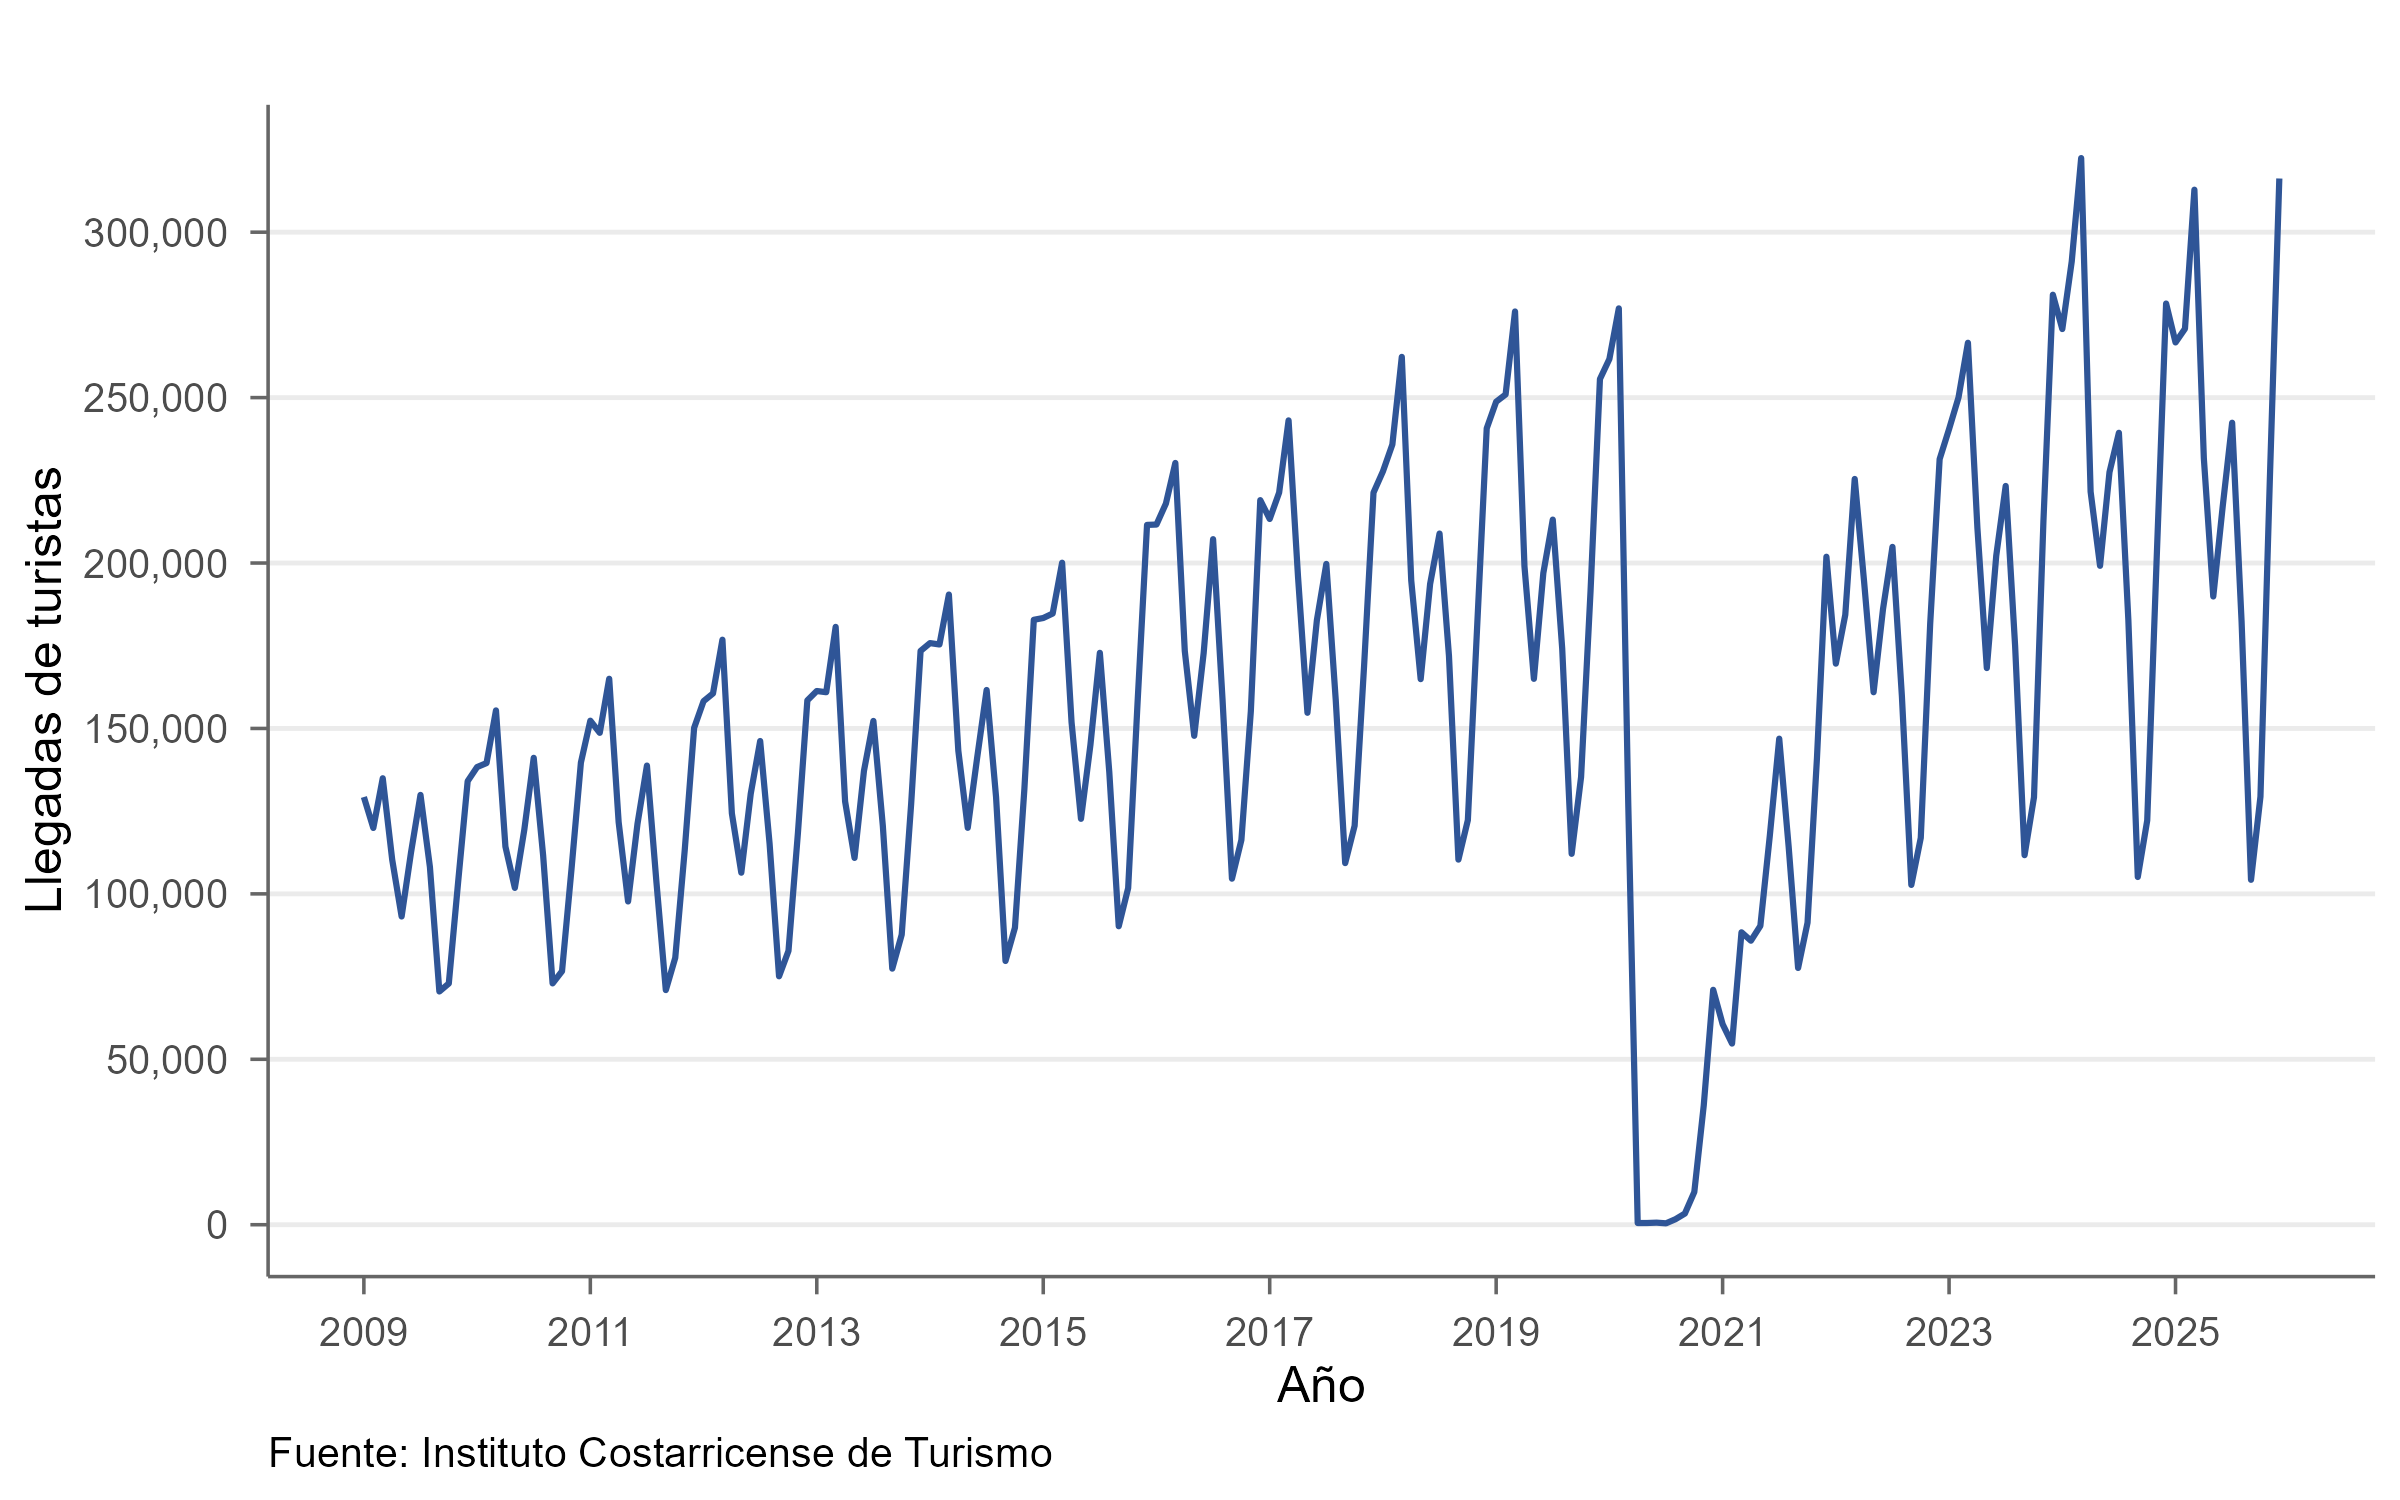
\includegraphics[width=0.85\textwidth]{figura2.png}
    \caption{Llegadas mensuales de turistas por vía 
    aérea en Costa Rica, 2009--2025.}
    \label{fig:serie}
\end{figure}

La Figura \ref{fig:estacionalidad} evidencia un patrón 
estacional anual, con mayores niveles de visitación 
entre enero y marzo, un repunte durante junio y julio 
y menores niveles en septiembre y octubre. Asimismo, 
la amplitud de las fluctuaciones estacionales tiende 
a aumentar con el nivel de la serie, lo que sugiere 
una estructura multiplicativa.

\begin{figure}[htbp]
    \centering
    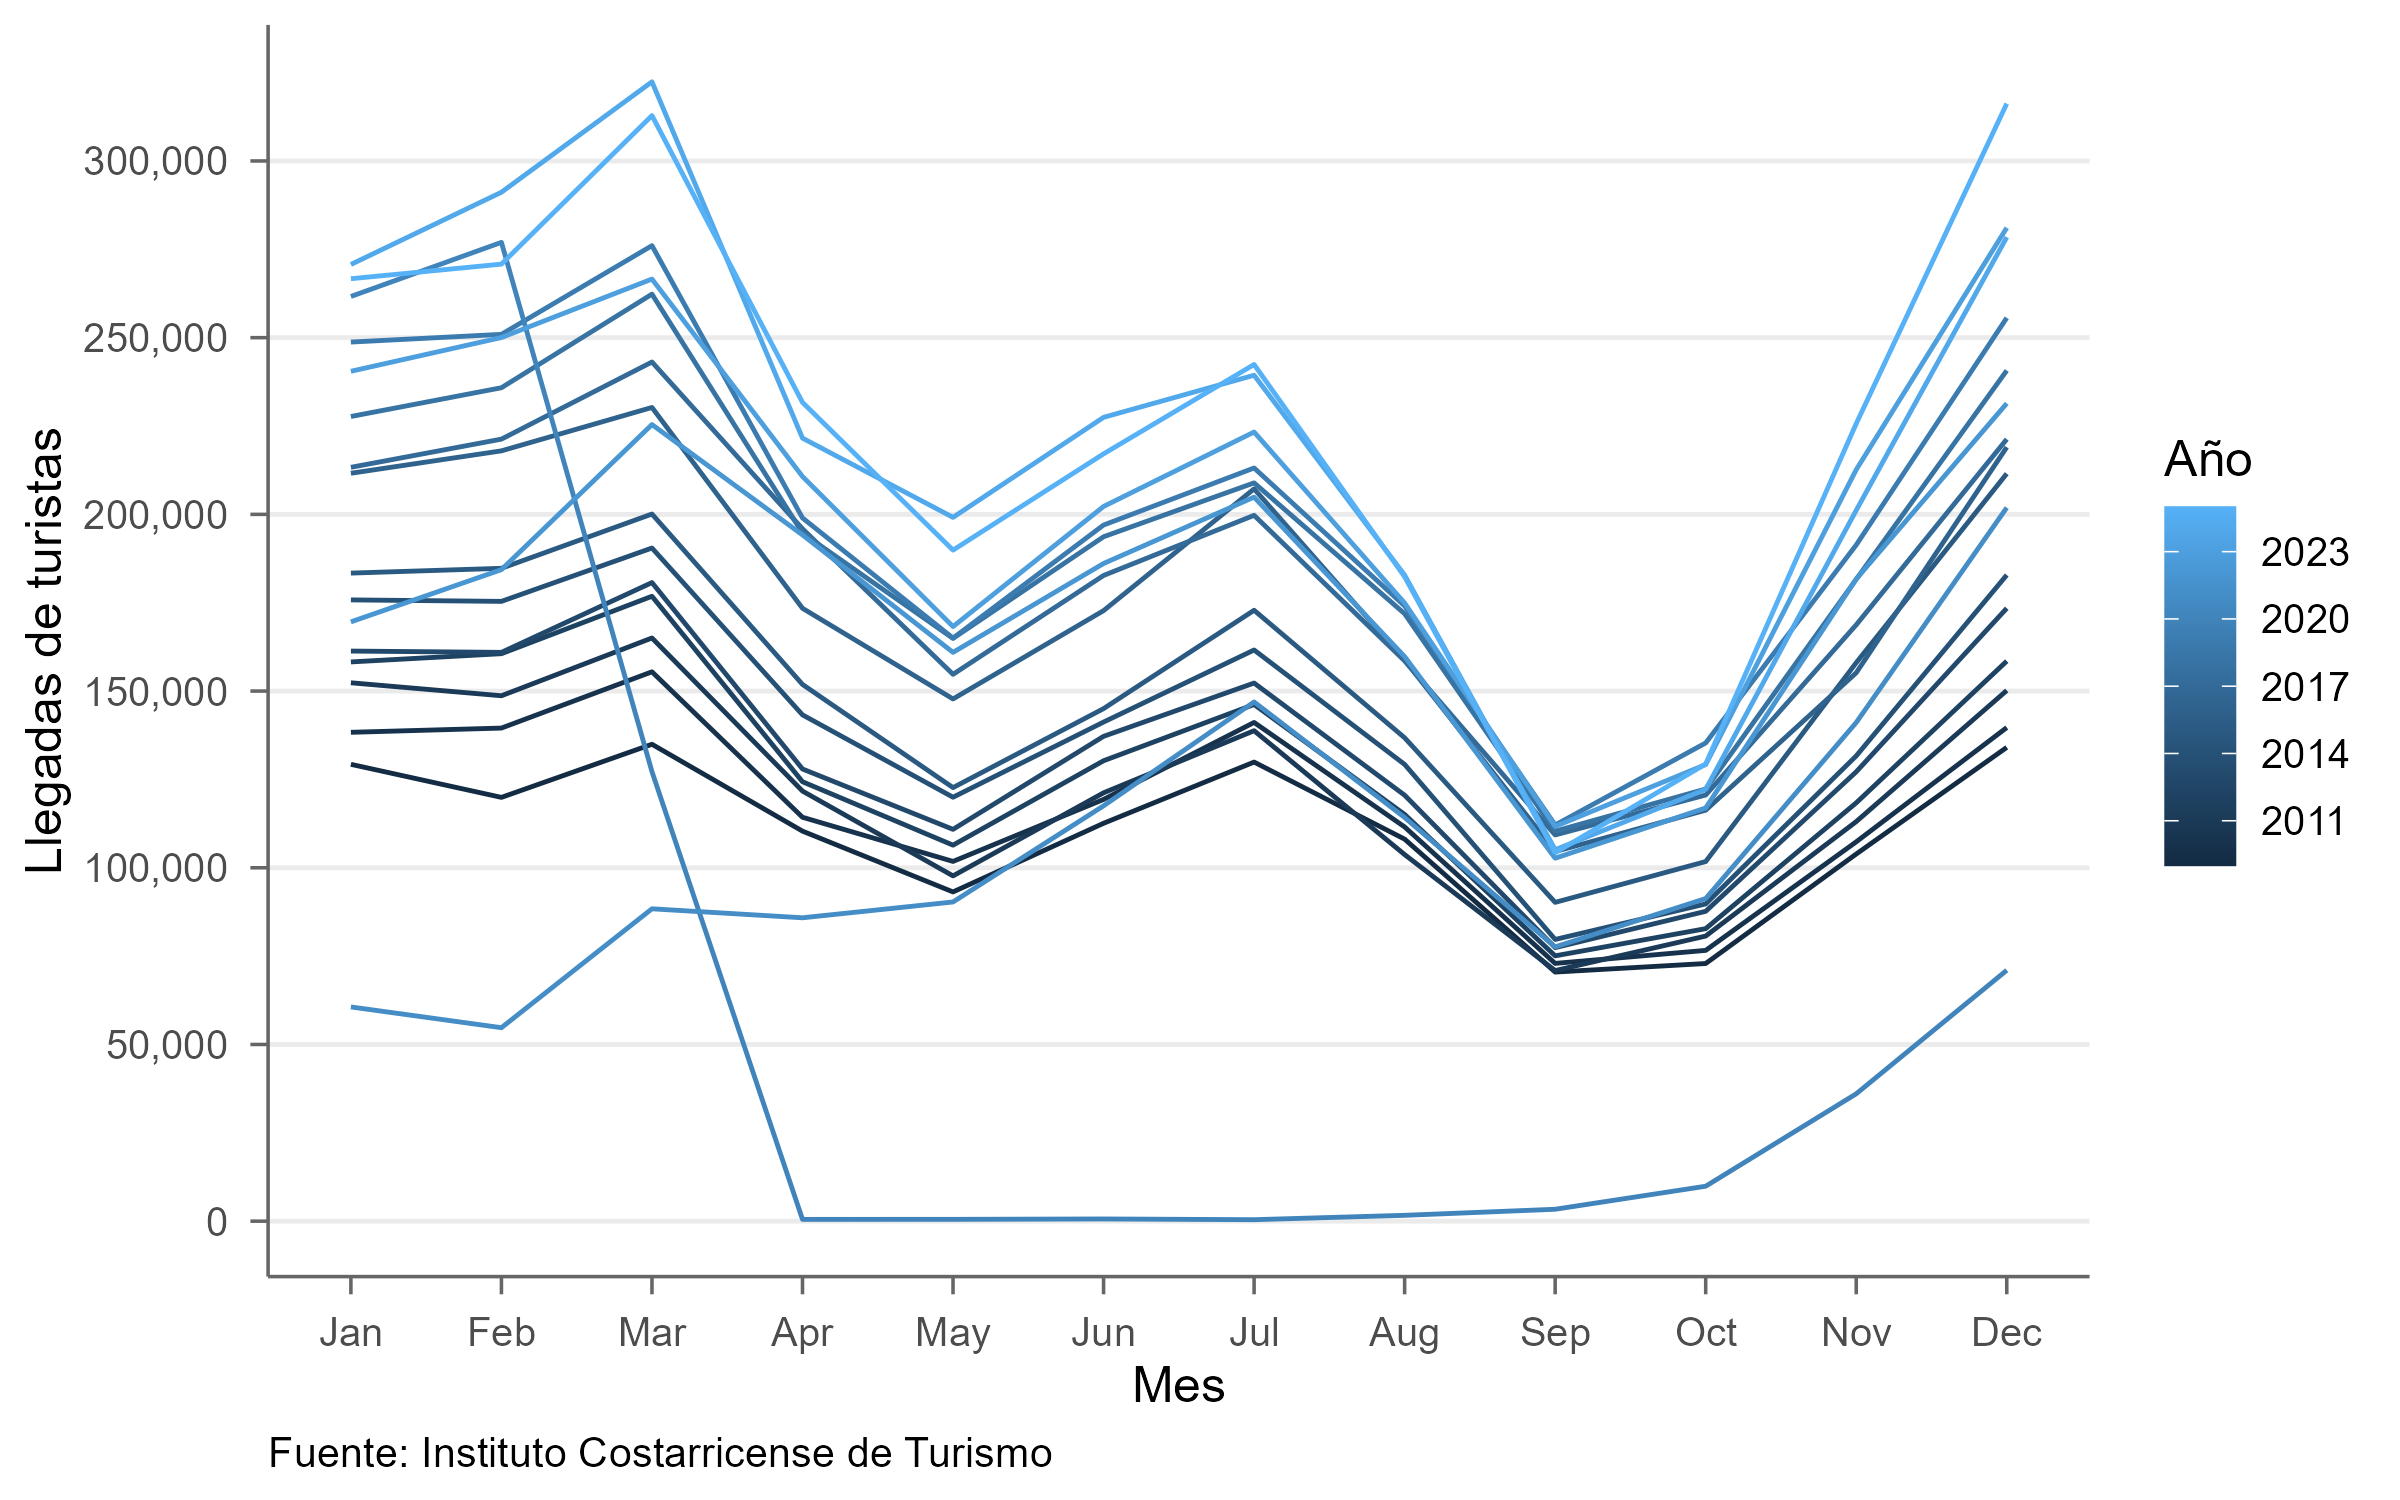
\includegraphics[width=0.85\textwidth]{figura3.png}
    \caption{Patrón estacional de las llegadas mensuales 
    de turistas por vía aérea en Costa Rica.}
    \label{fig:estacionalidad}
\end{figure}

La función de autocorrelación (Figura \ref{fig:acf}) 
presentó una autocorrelación cercana a 0,8 en el 
primer rezago y un incremento alrededor del rezago 12. 
Estos resultados, junto con la descomposición 
multiplicativa, justificaron la consideración de 
modelos que incorporaran tendencia, estacionalidad 
y dependencia temporal.

\begin{figure}[H]
    \centering
    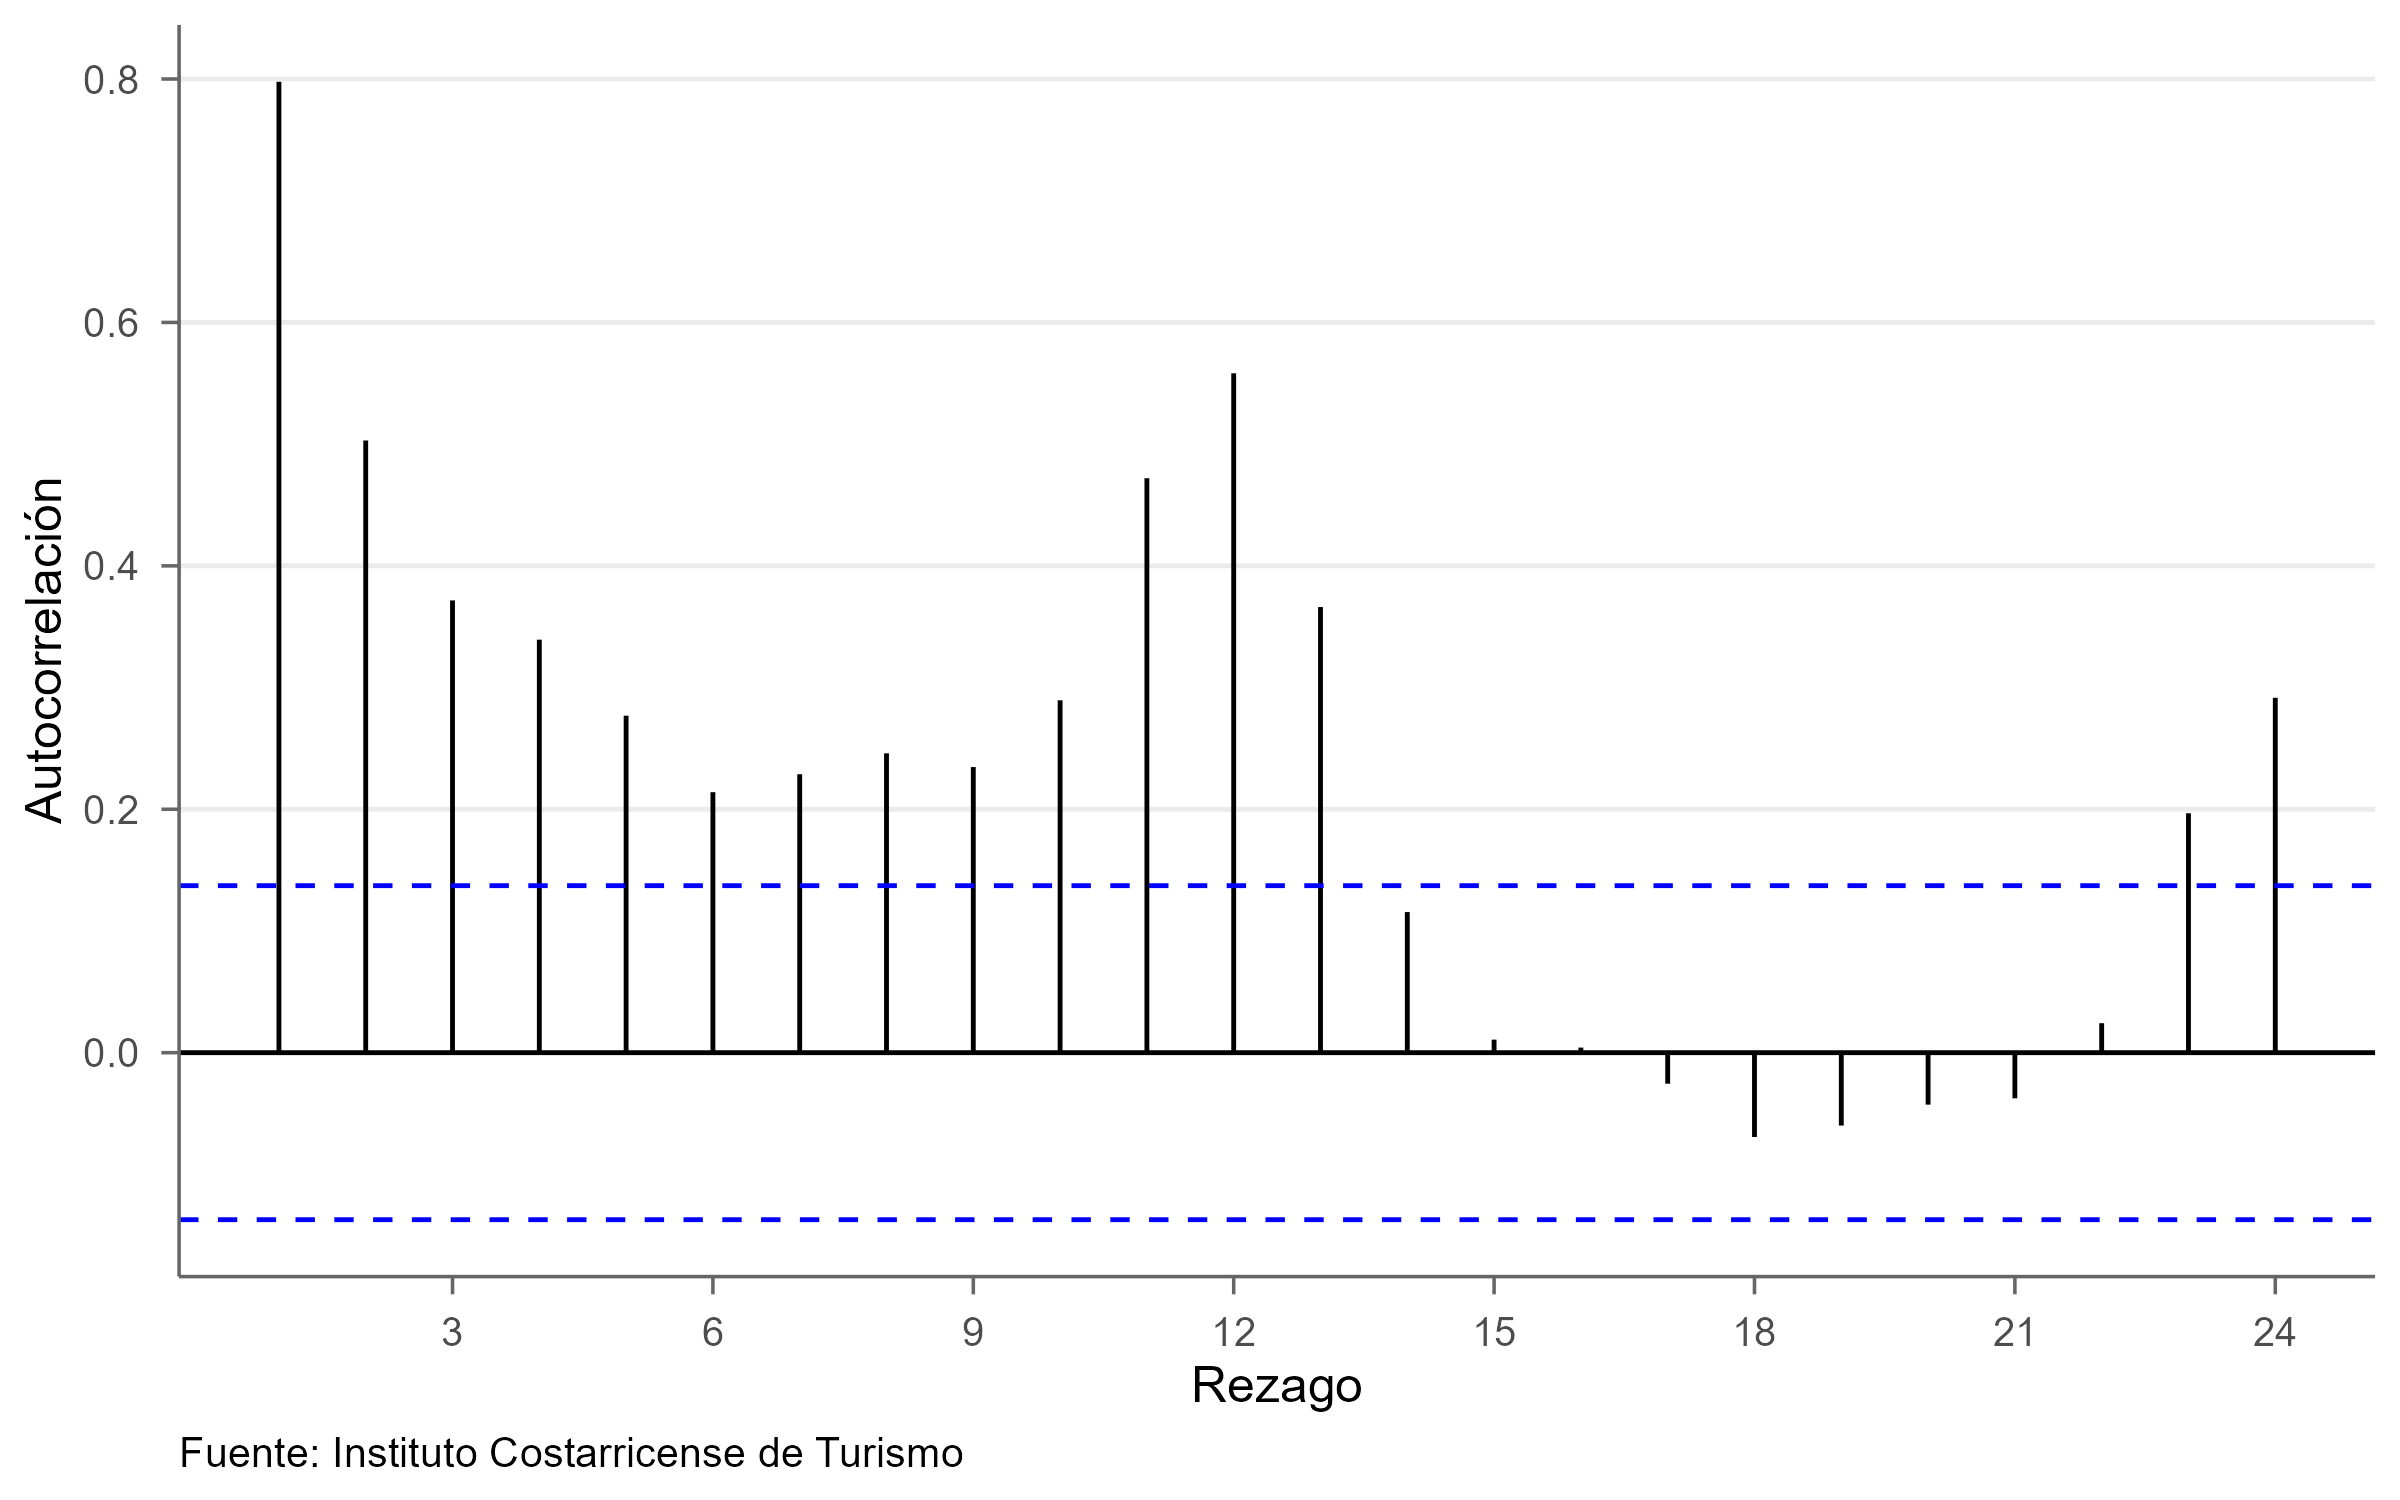
\includegraphics[width=0.85\textwidth]{figura5.png}
    \caption{Función de autocorrelación de las llegadas 
    mensuales de turistas por vía aérea en Costa Rica.}
    \label{fig:acf}
\end{figure}


\subsection{Selección de modelos finalistas}

\subsubsection{Suavizamiento exponencial}

Se evaluaron tres especificaciones del método 
Holt-Winters: aditivo, multiplicativo y multiplicativo 
con tendencia amortiguada. Se seleccionó el modelo 
aditivo, debido a que presentó los menores valores 
de AICc (4814,33) y BIC (4866,19), así como una menor 
autocorrelación residual en el primer rezago (0,232).

Los parámetros de suavizamiento estimados fueron:

\begin{equation}
\widehat{\alpha}=0{,}9999,\quad
\widehat{\beta}=0{,}0001,\quad
\widehat{\gamma}=0{,}0001.
\end{equation}

El valor de $\alpha$ cercano a uno indica que el nivel 
del modelo responde principalmente a las observaciones 
más recientes, mientras que los valores de $\beta$ y 
$\gamma$ cercanos a cero indican que los componentes 
de tendencia y estacionalidad presentan poca 
actualización a lo largo del tiempo.

Aunque el modelo multiplicativo amortiguado presentó 
menores errores durante el entrenamiento, se prefirió 
el modelo aditivo considerando los criterios de 
información y el comportamiento de los residuos. 
Sin embargo, la prueba de Ljung-Box resultó 
estadísticamente significativa ($p<0,001$), lo que 
indica que el modelo no logró representar completamente 
la dependencia temporal de la serie.

\subsubsection{Modelos ARIMA/SARIMA}

Para la modelación ARIMA/SARIMA se utilizó la serie 
transformada logarítmicamente. La prueba de Dickey-Fuller 
aumentada permitió rechazar la hipótesis nula de raíz 
unitaria ordinaria ($p=0,0109$), por lo que se consideraron 
modelos sin diferenciación ordinaria ($d=0$).

En la Figura \ref{fig:acf_pacf_sarima} se presentan las 
funciones de autocorrelación y autocorrelación parcial 
de la serie transformada. Se observa una autocorrelación 
elevada en los primeros rezagos, seguida de una disminución 
gradual, lo que motivó la evaluación de componentes 
autorregresivos.

\begin{figure}[H]
    \centering
    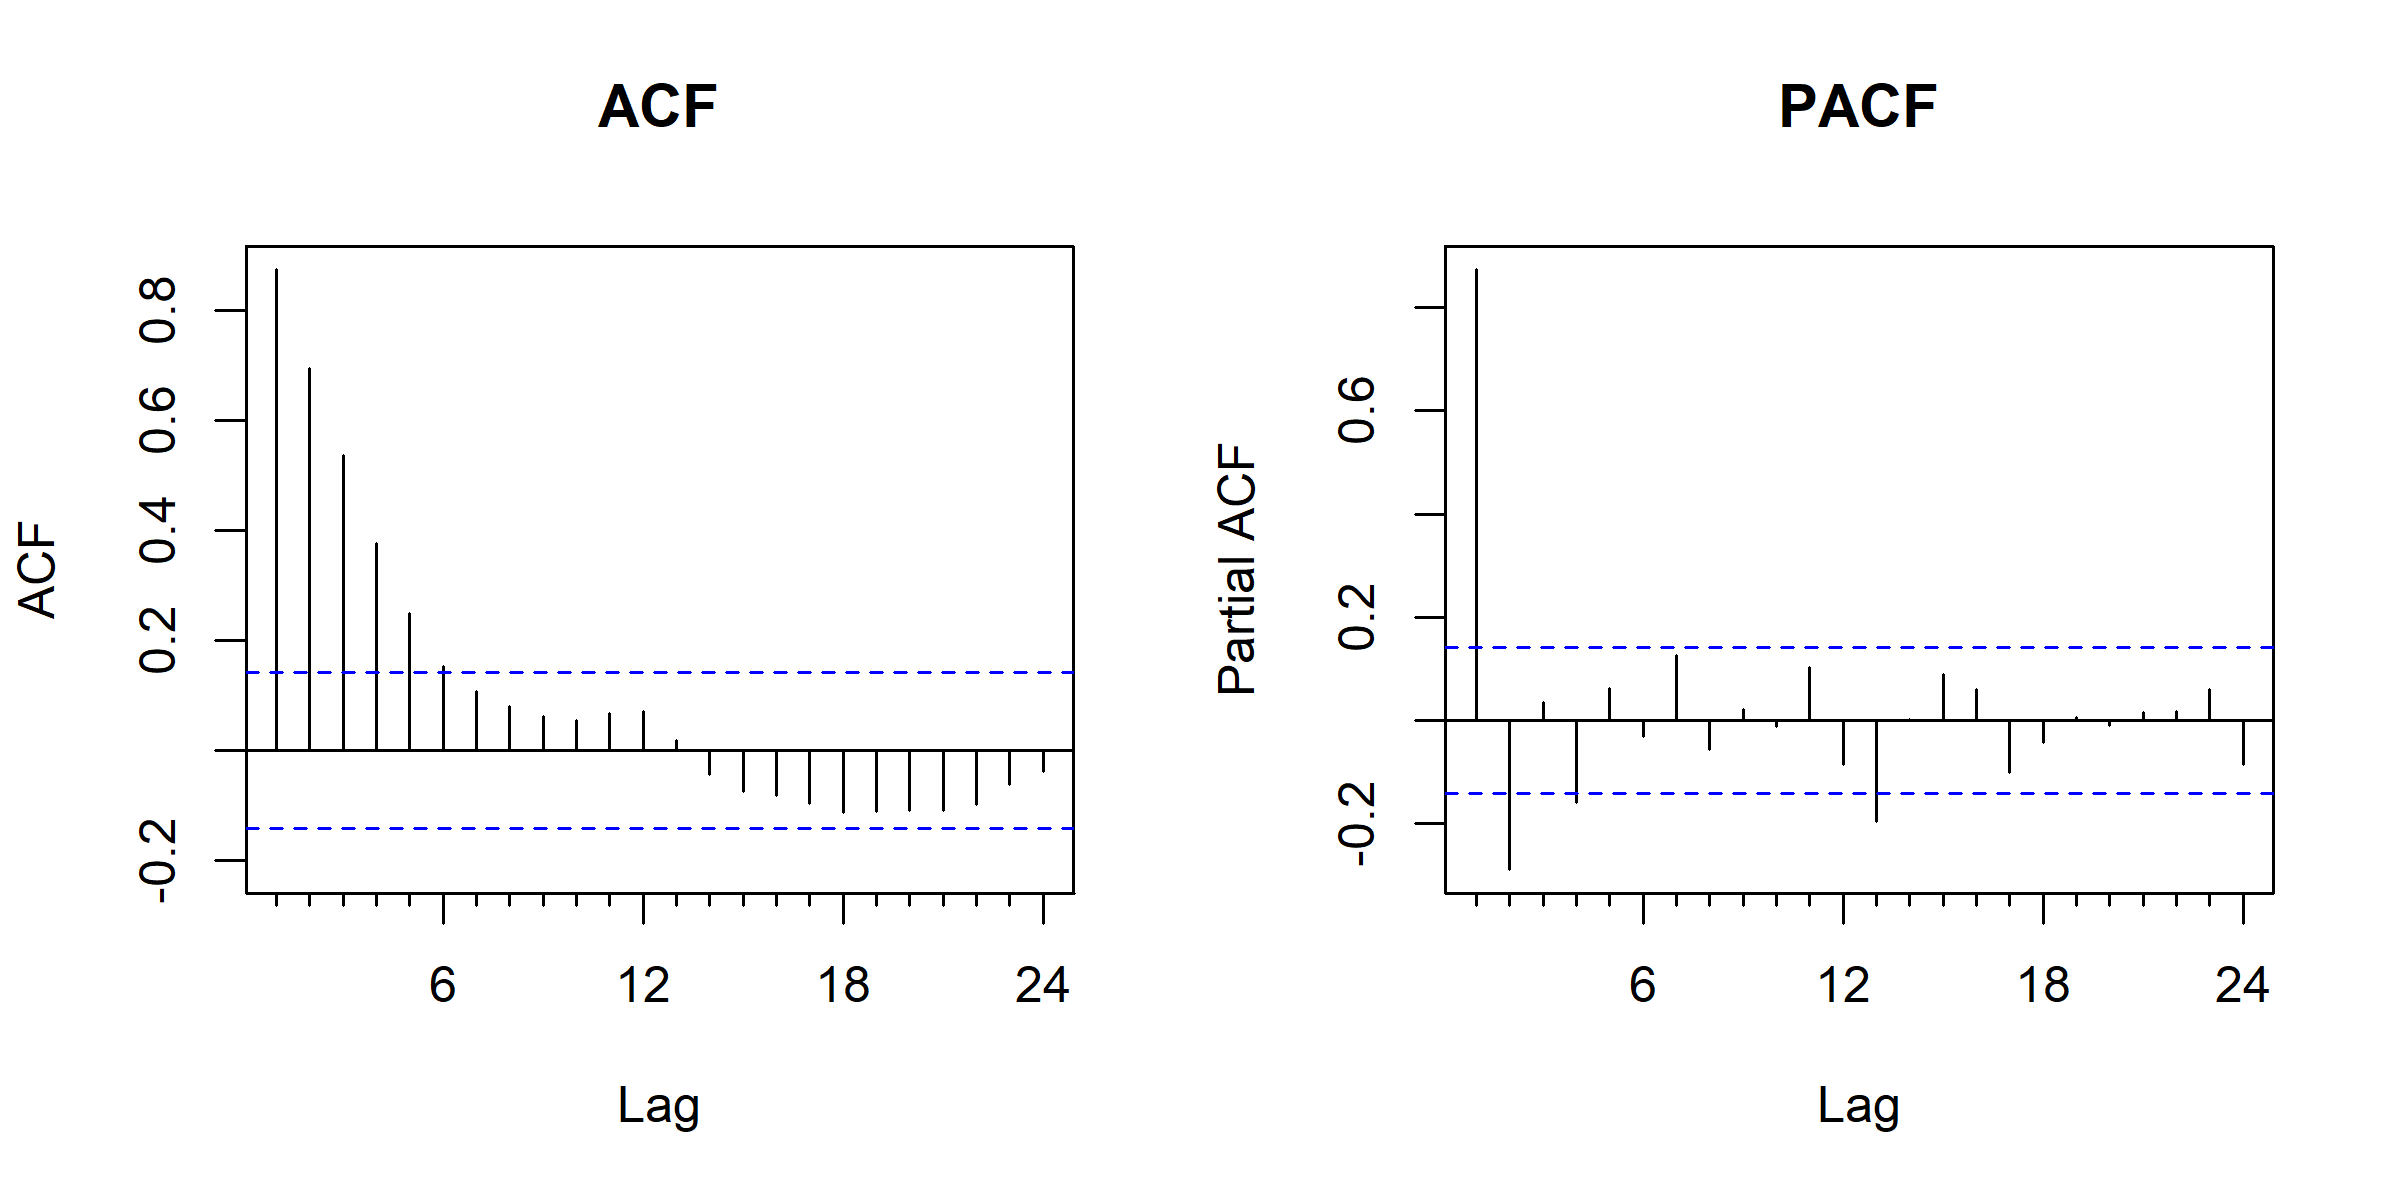
\includegraphics[width=0.85\textwidth]{figura7.png}
    \caption{Funciones de autocorrelación (ACF) y 
    autocorrelación parcial (PACF) de la serie 
    transformada logarítmicamente, sin diferenciación.}
    \label{fig:acf_pacf_sarima}
\end{figure}

También se evaluaron especificaciones con diferenciación 
estacional ($D=1$). Sin embargo, algunos de estos modelos 
presentaron parámetros de medias móviles en los límites 
de invertibilidad, por lo que se consideraron alternativas 
sin diferenciación estacional.

Finalmente, se seleccionó el modelo 
SARIMA$(2,0,0)(1,0,0)_{12}$, considerando su parsimonia, 
sus criterios de información (AICc de 250,06 y BIC de 
266,03) y los resultados del diagnóstico residual. 
La prueba de Ljung-Box no mostró evidencia estadística 
suficiente de autocorrelación residual ($p=0,5772$).

La ecuación del modelo estimado sobre el conjunto 
de entrenamiento está dada por:

\begin{equation}
\begin{aligned}
&(1-1{,}1403B+0{,}2942B^2)\\
&\quad(1-0{,}2078B^{12})(w_t-11{,}7554)=a_t.
\end{aligned}
\label{eq:sarima_estimado}
\end{equation}

donde $w_t=\ln(Y_t)$, $B$ representa el operador de 
rezago y $a_t$ corresponde a las innovaciones del modelo.

\subsubsection{Modelos de regresión}

Se evaluaron cuatro especificaciones de regresión, 
considerando tendencias lineales y cuadráticas, con 
y sin transformación logarítmica. Se seleccionó el 
modelo con tendencia lineal y variables indicadoras 
mensuales en la escala original, debido a que presentó 
el mayor coeficiente de determinación ajustado 
($R^2_{aj}=0{,}4386$). Además, la incorporación de un término 
cuadrático no produjo una mejora significativa en el 
ajuste ($p=0,7299$).

El modelo estimado sobre el conjunto de entrenamiento 
está dado por:

\begin{equation}
\widehat{Y}_t=152744{,}77+384{,}08t+
\sum_{j=2}^{12}\widehat{\gamma}_j I_{j,t}.
\label{eq:regresion_estimada}
\end{equation}

El coeficiente asociado con la tendencia indica un 
incremento estimado de aproximadamente 384 llegadas 
por mes, una vez considerados los efectos estacionales.

Sin embargo, la prueba de Breusch-Godfrey evidenció 
autocorrelación residual significativa ($p<0,001$), 
lo que indica que los componentes determinísticos de 
tendencia y estacionalidad no fueron suficientes para 
representar la dependencia temporal de la serie. Esta 
limitación motivó la consideración de modelos de 
regresión con errores ARIMA.

\subsubsection{Modelos de regresión dinámica}

Se evaluaron seis especificaciones de regresión 
dinámica, considerando diferentes estructuras ARIMA 
para los errores, transformaciones logarítmicas y 
variables de intervención asociadas con la pandemia 
por COVID-19.

Aunque algunas especificaciones con variables de 
intervención presentaron menores criterios de 
información y errores durante el entrenamiento, 
estas mostraron autocorrelación residual significativa. 
Por lo tanto, se seleccionó el modelo de regresión 
con tendencia lineal, estacionalidad mensual y errores 
ARIMA$(4,0,0)$, sin transformación logarítmica ni 
variables de intervención explícitas.

El modelo estimado sobre el conjunto de entrenamiento 
se expresa como:

\begin{equation}
Y_t=149048{,}36+464{,}03t+
\sum_{j=1}^{11}\widehat{\gamma}_j I_{j,t}+\eta_t.
\label{eq:dinamica_estimada}
\end{equation}

La estructura autorregresiva estimada para el término 
de error está dada por:

\begin{equation}
\begin{aligned}
\eta_t={}&1{,}2680\eta_{t-1}
-0{,}6047\eta_{t-2}\\
&+0{,}3914\eta_{t-3}
-0{,}1518\eta_{t-4}+a_t.
\end{aligned}
\label{eq:ar4_estimado}
\end{equation}

El modelo presentó un AICc de 4315,74, un BIC de 
4370,42 y un RMSE de entrenamiento de 16.483,25 
llegadas. Asimismo, la autocorrelación residual en 
el primer rezago fue cercana a cero (0,0154) y la 
prueba de Ljung-Box no mostró evidencia estadística 
suficiente de autocorrelación residual ($p=0,1377$).



\subsection{Comparación y selección del modelo definitivo}

Una vez seleccionado un representante de cada familia, 
se comparó la adecuación estadística y la capacidad 
predictiva de los cuatro modelos finalistas.

En la Tabla \ref{tab:diagnostico} se presentan los 
resultados de las pruebas de autocorrelación residual 
aplicadas a los modelos ajustados sobre el conjunto 
de entrenamiento.

\begin{table}[H]
    \centering
    \caption{Diagnóstico de autocorrelación residual 
    de los modelos finalistas.}
    \label{tab:diagnostico}
    \begin{tabular}{lcccc}
        \hline
        Modelo & Prueba & Estadístico & gl & Valor $p$ \\
        \hline
        Holt-Winters aditivo & LB & 67,078 & 24 & $<0,001$ \\
        SARIMA$(2,0,0)(1,0,0)_{12}$ & LB & 19,124 & 21 & 0,5772 \\
        Regresión convencional & BG & 169,130 & 24 & $<0,001$ \\
        Regresión dinámica & LB & 26,913 & 20 & 0,1377 \\
        \hline
    \end{tabular}

    \begin{flushleft}
        \footnotesize
        Nota: LB = Ljung-Box; BG = Breusch-Godfrey;
        gl = grados de libertad.
        Fuente: elaboración propia.
    \end{flushleft}
\end{table}

Los modelos SARIMA y de regresión dinámica no 
presentaron evidencia estadísticamente significativa 
de autocorrelación residual, a diferencia de los modelos 
Holt-Winters aditivo y de regresión convencional. 

Por otra parte, la prueba de Shapiro-Wilk permitió 
rechazar la hipótesis de normalidad de los residuos 
en los cuatro modelos finalistas ($p<0,05$). Este 
resultado podría estar relacionado con las alteraciones 
extraordinarias registradas durante la pandemia por 
COVID-19.

Si bien la falta de normalidad constituye una limitación 
para la construcción de intervalos de predicción 
basados en supuestos gaussianos, no implica necesariamente 
una menor precisión de los pronósticos puntuales. Por 
lo tanto, se conservaron los cuatro modelos finalistas 
para evaluar su capacidad predictiva fuera de muestra.

Para dicha evaluación se generaron pronósticos 
correspondientes a los 12 meses del año 2025. 
En la Tabla \ref{tab:comparacion} se presentan 
las medidas de precisión predictiva obtenidas 
sobre el conjunto de prueba.

\begin{table}[H]
    \centering
    \caption{Comparación de la capacidad predictiva 
    de los modelos finalistas fuera de muestra.}
    \label{tab:comparacion}
    \begin{tabular}{lrrrr}
        \hline
        Modelo & RMSE & MAE & MAPE (\%) & MASE \\
        \hline
        Holt-Winters aditivo 
        & 36.776,39 & 29.411,93 & 18,36 & 0,9268 \\
        SARIMA 
        & 65.345,28 & 48.916,79 & 20,45 & 1,5414 \\
        Regresión convencional 
        & 42.379,74 & 36.967,81 & 15,60 & 1,1649 \\
        Regresión dinámica 
        & \textbf{26.617,18} & \textbf{19.898,07} 
        & \textbf{10,55} & \textbf{0,6270} \\
        \hline
    \end{tabular}

    \begin{flushleft}
        \footnotesize
        Nota: Los valores en negrita corresponden 
        al mejor resultado de cada medida. 
        Fuente: elaboración propia.
    \end{flushleft}
\end{table}

El modelo de regresión dinámica presentó el mejor 
desempeño predictivo en las cuatro medidas evaluadas, 
con un RMSE de 26.617,18 llegadas y un MAPE de 
10,55\,\%. En términos de RMSE, este modelo logró 
una reducción del 27,62\,\% respecto al método 
aditivo de Holt-Winters, del 59,27\,\% respecto al 
modelo SARIMA y del 37,19\,\% respecto a la 
regresión convencional.

Asimismo, el MASE obtenido fue de 0,6270, lo que 
indica que el error absoluto medio del modelo 
representó aproximadamente el 62,7\,\% del error 
absoluto medio del método ingenuo estacional 
calculado sobre el conjunto de entrenamiento.

\begin{figure}[H]
    \centering
    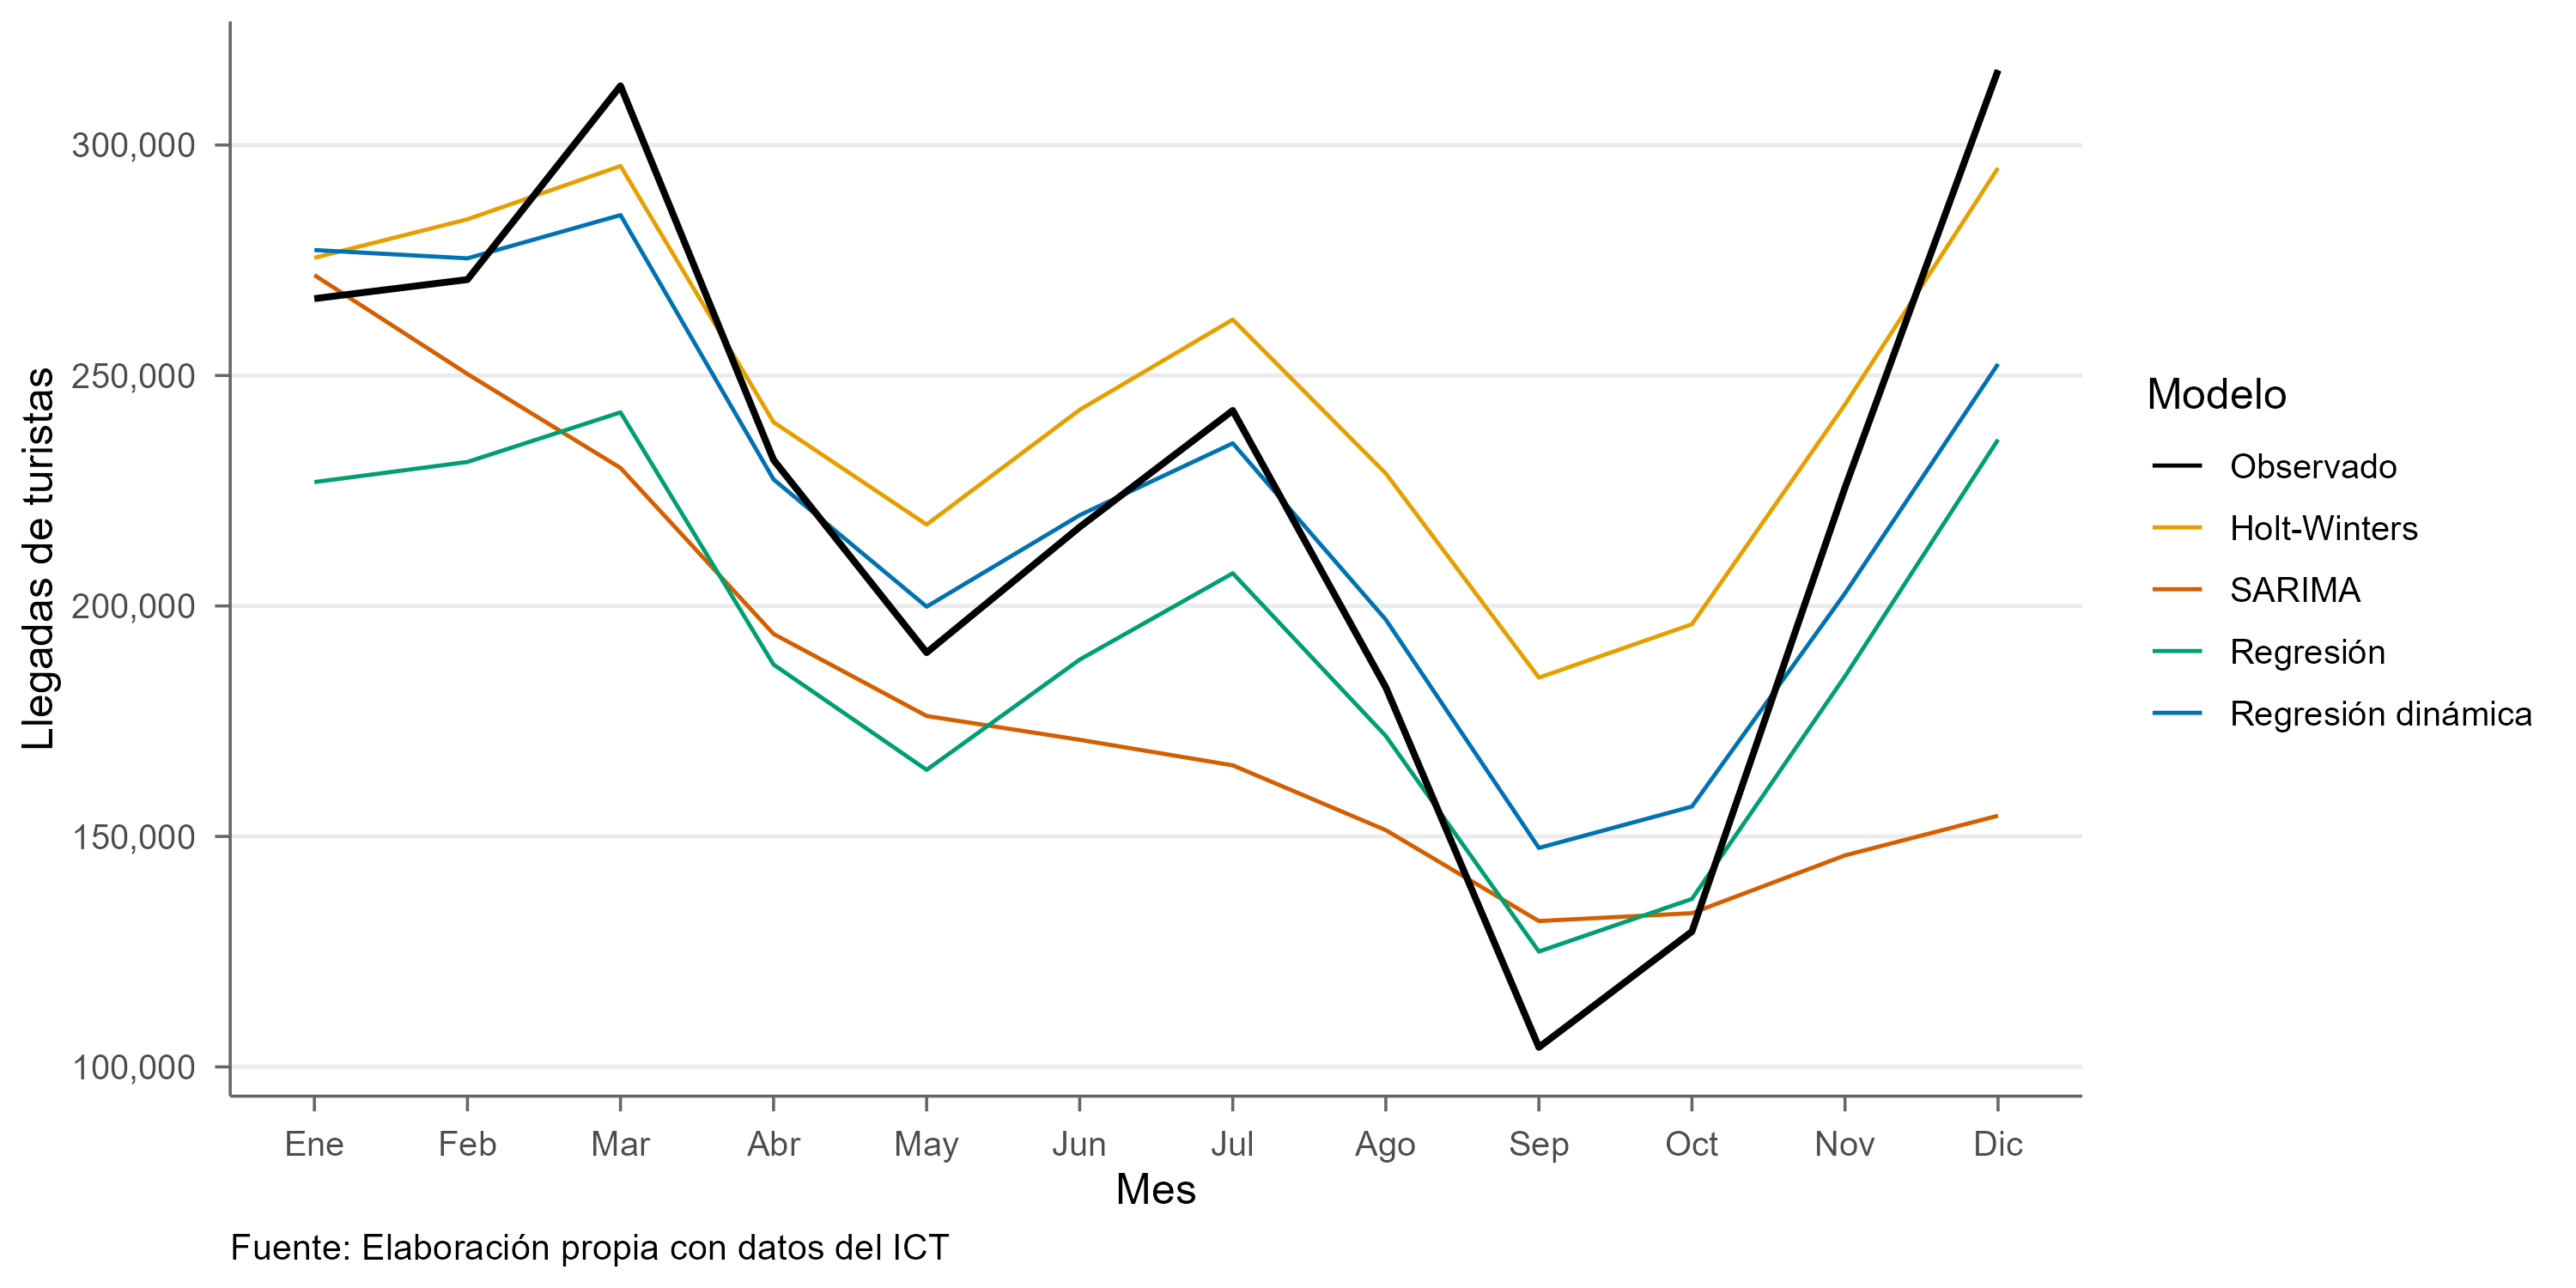
\includegraphics[width=0.95\textwidth]{figura8.png}
    \caption{Comparación de los pronósticos de los 
    cuatro modelos finalistas frente a las llegadas 
    observadas durante 2025.}
    \label{fig:comparacion}
\end{figure}

En la Figura \ref{fig:comparacion} se observa que el 
modelo aditivo de Holt-Winters tiende a sobreestimar 
las llegadas durante buena parte del año, mientras que 
los modelos SARIMA y de regresión convencional presentan 
subestimaciones en los meses de mayor visitación.

Por su parte, la regresión dinámica muestra, en términos 
generales, una mayor proximidad a los valores observados, 
aunque presenta dificultades para representar la magnitud 
de la disminución en septiembre y el incremento en 
diciembre.

Considerando su superioridad en las cuatro medidas de 
precisión predictiva y los resultados favorables del 
diagnóstico residual, se seleccionó el modelo de 
regresión dinámica con errores ARIMA$(4,0,0)$ para 
la generación de pronósticos.

\subsection{Reestimación y diagnóstico del modelo definitivo}

Una vez seleccionado el modelo de regresión dinámica 
con errores ARIMA$(4,0,0)$, se reestimaron sus parámetros 
utilizando las 204 observaciones disponibles, con el 
propósito de incorporar la información más reciente 
para la generación de pronósticos.

El modelo definitivo está dado por:

\begin{equation}
Y_t=146734{,}57+528{,}68t+
\sum_{j=1}^{11}\widehat{\gamma}_j I_{j,t}+\eta_t,
\label{eq:modelo_definitivo}
\end{equation}

donde el término de error sigue un proceso 
autorregresivo de orden cuatro:

\begin{equation}
\begin{aligned}
\eta_t={}&1{,}2831\eta_{t-1}
-0{,}6510\eta_{t-2}\\
&+0{,}4268\eta_{t-3}
-0{,}1572\eta_{t-4}+a_t.
\end{aligned}
\label{eq:ar4_definitivo}
\end{equation}

En la Tabla \ref{tab:coeficientes_finales} se presentan 
los coeficientes estimados del modelo definitivo.

\begin{table}[H]
    \centering
    \caption{Coeficientes estimados del modelo definitivo
    de regresión dinámica.}
    \label{tab:coeficientes_finales}
    \begin{tabular}{lr lr}
        \hline
        Parámetro & Estimación & Parámetro & Estimación \\
        \hline
        Intercepto & 146.734,57 & Junio & $-45.693,92$ \\
        Tendencia & 528,68 & Julio & $-27.485,56$ \\
        Enero & $-1.606,90$ & Agosto & $-65.118,29$ \\
        Febrero & 1.513,62 & Septiembre & $-114.591,47$ \\
        Marzo & 13.317,00 & Octubre & $-103.309,74$ \\
        Abril & $-43.814,23$ & Noviembre & $-53.044,41$ \\
        Mayo & $-68.812,51$ & Diciembre & Referencia \\
        \hline
        $\phi_1$ & 1,2831 & $\phi_3$ & 0,4268 \\
        $\phi_2$ & $-0,6510$ & $\phi_4$ & $-0,1572$ \\
        \hline
    \end{tabular}

    \begin{flushleft}
        \footnotesize
        Nota: Diciembre corresponde a la categoría de 
        referencia de las variables indicadoras 
        estacionales. Fuente: elaboración propia.
    \end{flushleft}
\end{table}

El coeficiente asociado con la tendencia indica un 
incremento estimado de aproximadamente 529 llegadas 
por mes, una vez considerados los efectos estacionales. 
Respecto a diciembre, marzo presenta el mayor efecto 
estacional positivo, mientras que septiembre y octubre 
presentan las mayores disminuciones, lo que resulta 
consistente con el comportamiento identificado durante 
el análisis exploratorio.

El diagnóstico residual del modelo definitivo presentó 
una autocorrelación de primer orden cercana a cero 
(0,0129). Asimismo, la prueba de Ljung-Box obtuvo un 
estadístico de 23,538, con 20 grados de libertad y 
un valor $p$ de 0,2631, por lo que no se encontró 
evidencia estadística suficiente de autocorrelación 
residual hasta los rezagos evaluados.

\begin{figure}[H]
    \centering
    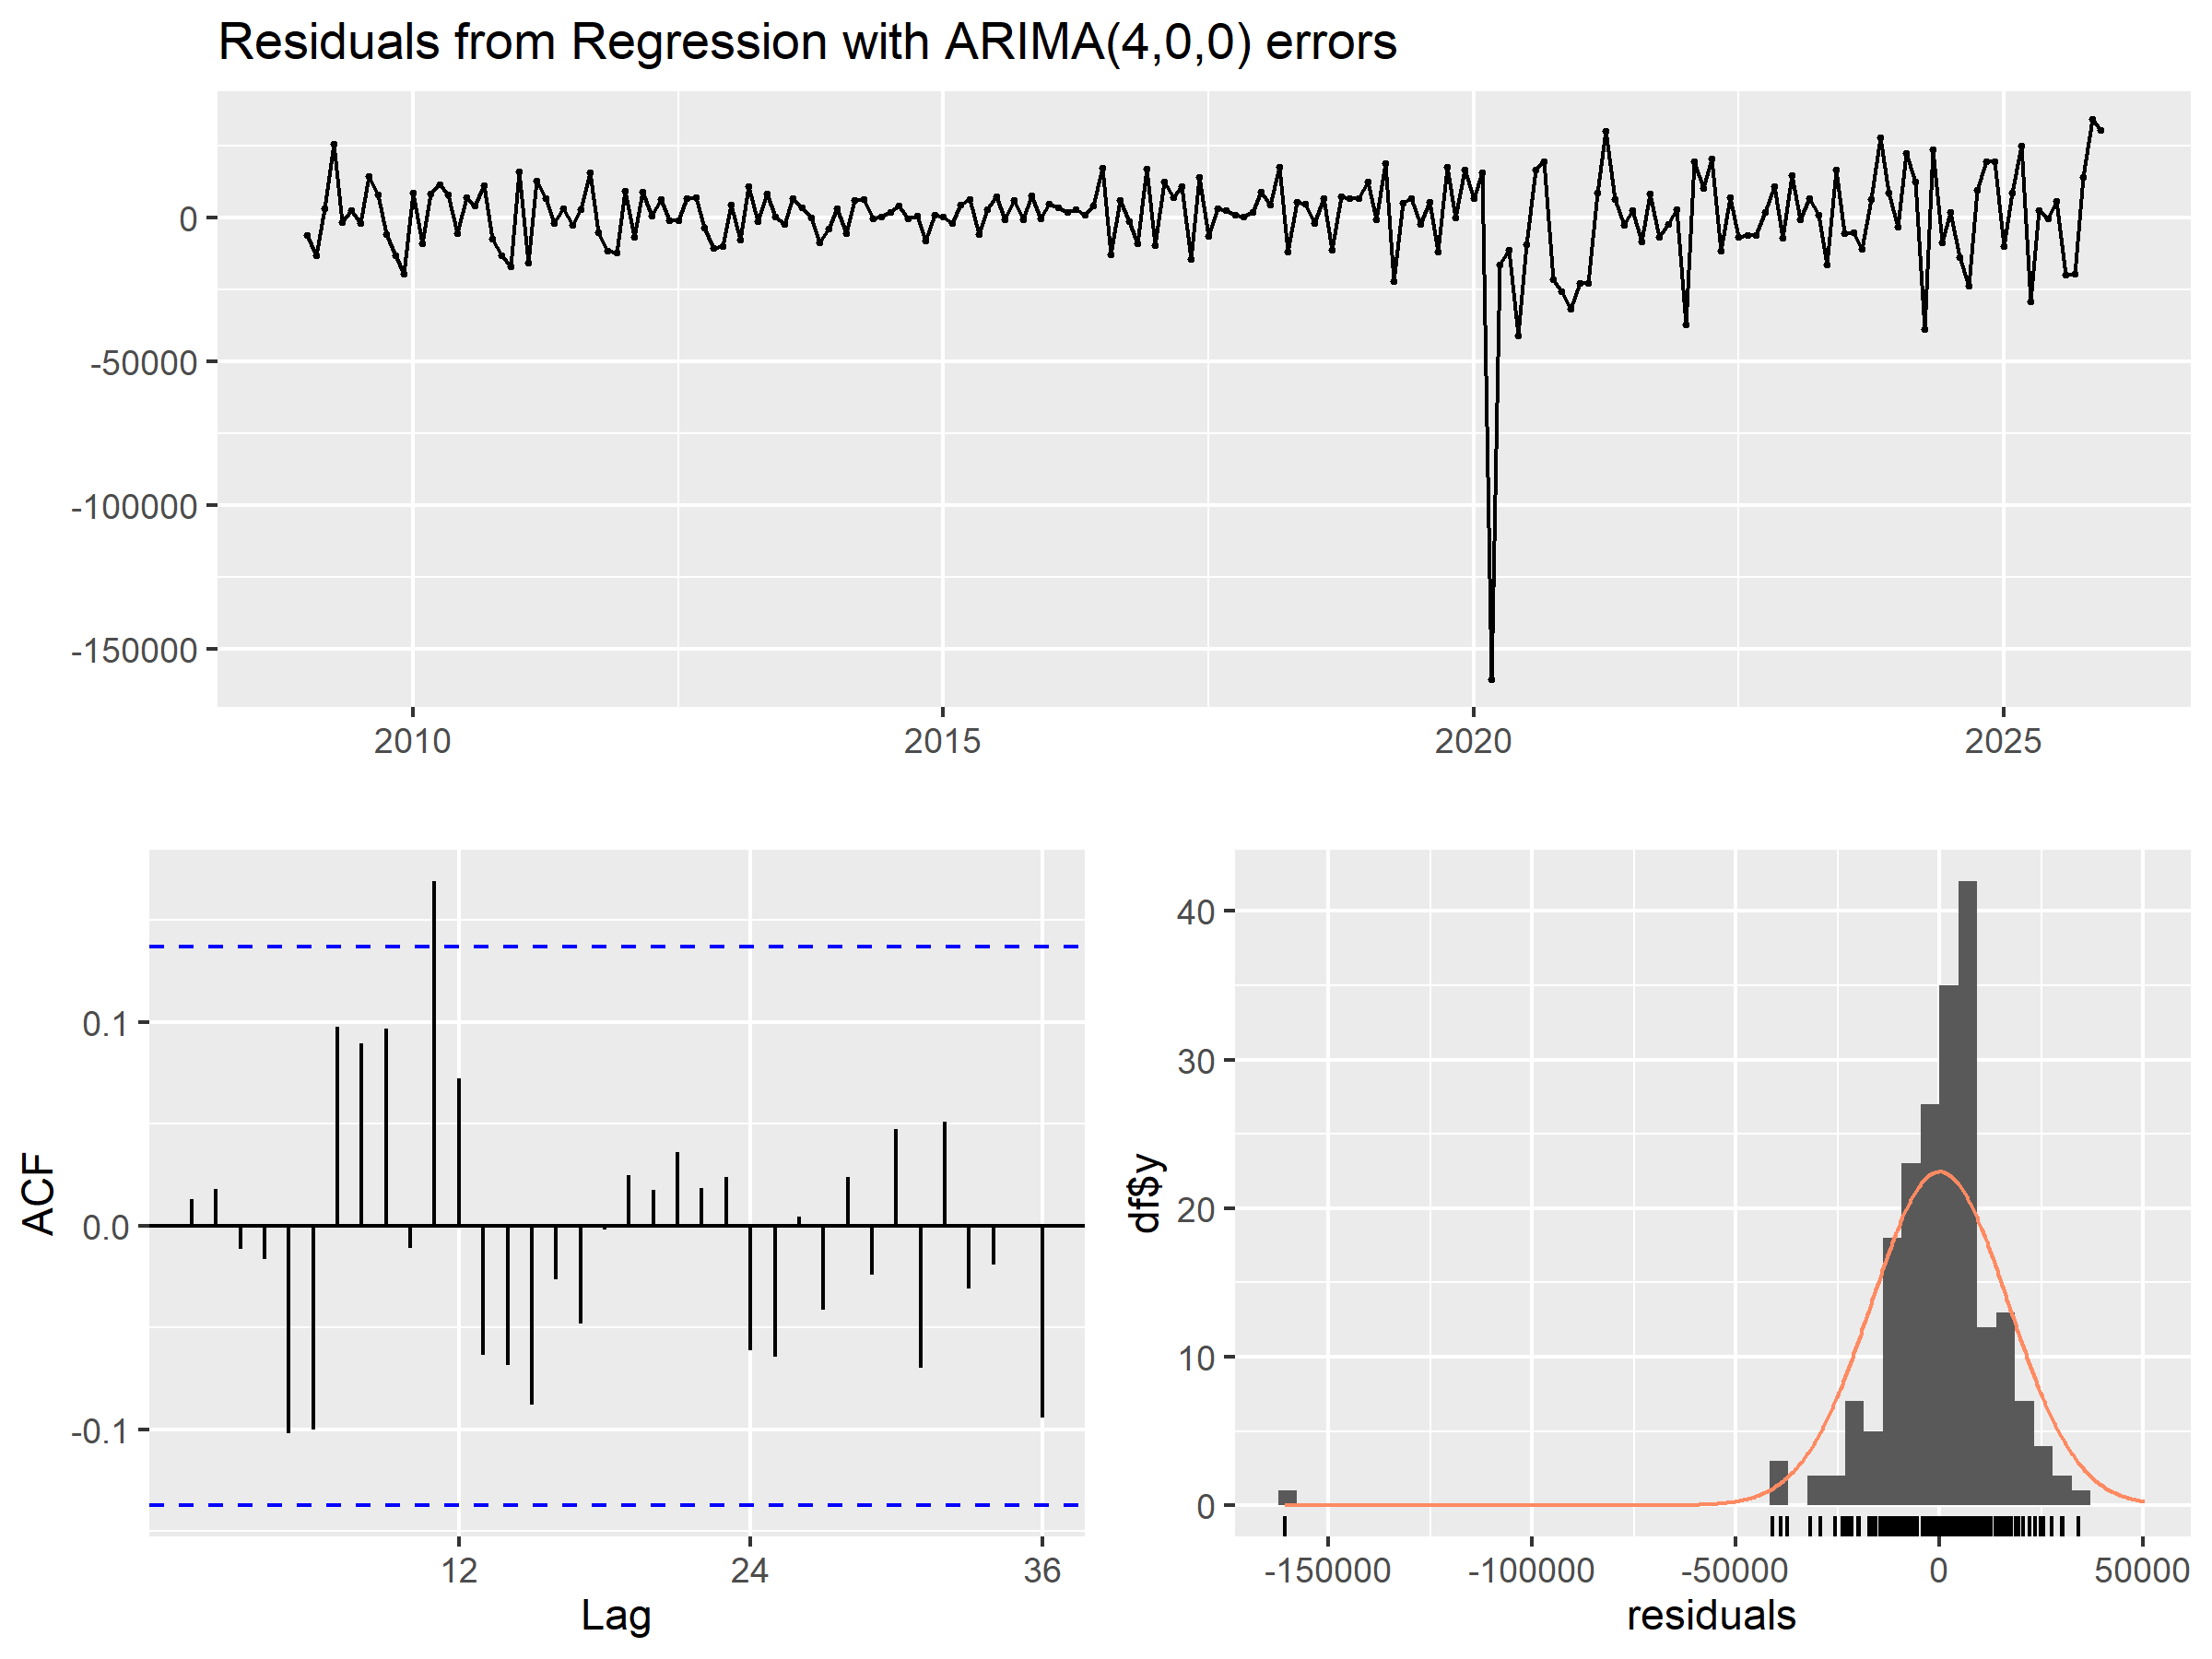
\includegraphics[width=0.90\textwidth]{figura9.png}
    \caption{Diagnóstico de residuos del modelo 
    definitivo de regresión dinámica.}
    \label{fig:residuos_final}
\end{figure}

En la Figura \ref{fig:residuos_final} se observa que 
los residuos fluctúan alrededor de cero y que la 
mayoría de las autocorrelaciones se encuentran dentro 
de los límites de significancia. Sin embargo, se 
identifican valores extremos negativos durante 2020, 
asociados con la pandemia por COVID-19, así como 
cambios en la variabilidad de los residuos.

La prueba de Shapiro-Wilk obtuvo un estadístico 
$W=0{,}7282$ y un valor $p<0.01$, 
por lo que se rechazó la hipótesis de normalidad. 
Este resultado es consistente con la asimetría 
negativa observada en el histograma.

Aunque estas características no invalidan 
necesariamente los pronósticos puntuales, constituyen 
una limitación del modelo y requieren cautela en 
la interpretación de los intervalos de predicción.



\subsection{Pronósticos para 2026}

A partir del modelo definitivo de regresión dinámica 
con errores ARIMA$(4,0,0)$, se generaron pronósticos 
para los doce meses de 2026, acompañados de intervalos 
de predicción del 80\,\% y 95\,\%. Los resultados se 
presentan en la Tabla \ref{tab:pronosticos2026}.

\begin{table}[H]
    \centering
    \caption{Pronósticos mensuales de llegadas de 
    turistas por vía aérea para 2026.}
    \label{tab:pronosticos2026}
    \begin{tabular}{lrrrrr}
        \hline
        & & \multicolumn{2}{c}{IP 80\,\%} 
        & \multicolumn{2}{c}{IP 95\,\%} \\
        \cline{3-6}
        Mes & Pronóstico & Inferior & Superior 
        & Inferior & Superior \\
        \hline
        Enero      & 313.013 & 290.584 & 335.442 & 278.711 & 347.315 \\
        Febrero    & 307.184 & 270.698 & 343.671 & 251.383 & 362.986 \\
        Marzo      & 317.368 & 274.594 & 360.141 & 251.951 & 382.785 \\
        Abril      & 257.453 & 210.452 & 304.454 & 185.571 & 329.335 \\
        Mayo       & 226.423 & 175.646 & 277.201 & 148.766 & 304.081 \\
        Junio      & 244.383 & 190.843 & 297.924 & 162.500 & 326.266 \\
        Julio      & 259.018 & 203.658 & 314.377 & 174.352 & 343.683 \\
        Agosto     & 218.074 & 161.397 & 274.750 & 131.394 & 304.753 \\
        Septiembre & 165.477 & 107.810 & 223.144 & 77.282  & 253.672 \\
        Octubre    & 174.245 & 115.866 & 232.624 & 84.962  & 263.528 \\
        Noviembre  & 222.519 & 163.634 & 281.404 & 132.462 & 312.576 \\
        Diciembre  & 273.884 & 214.631 & 333.138 & 183.264 & 364.505 \\
        \hline
        \textbf{Total} & \textbf{2.979.040} & -- & -- & -- & -- \\
        \hline
    \end{tabular}

    \begin{flushleft}
        \footnotesize
        Nota: IP = intervalo de predicción. 
        Fuente: elaboración propia.
    \end{flushleft}
\end{table}

El total anual pronosticado fue de aproximadamente 
2.979.040 llegadas de turistas por vía aérea. Marzo 
presentó el mayor número de llegadas pronosticadas 
(317.368), mientras que septiembre registró el menor 
valor (165.477). Este comportamiento es consistente 
con el patrón estacional identificado durante el 
análisis exploratorio.

\begin{figure}[H]
    \centering
    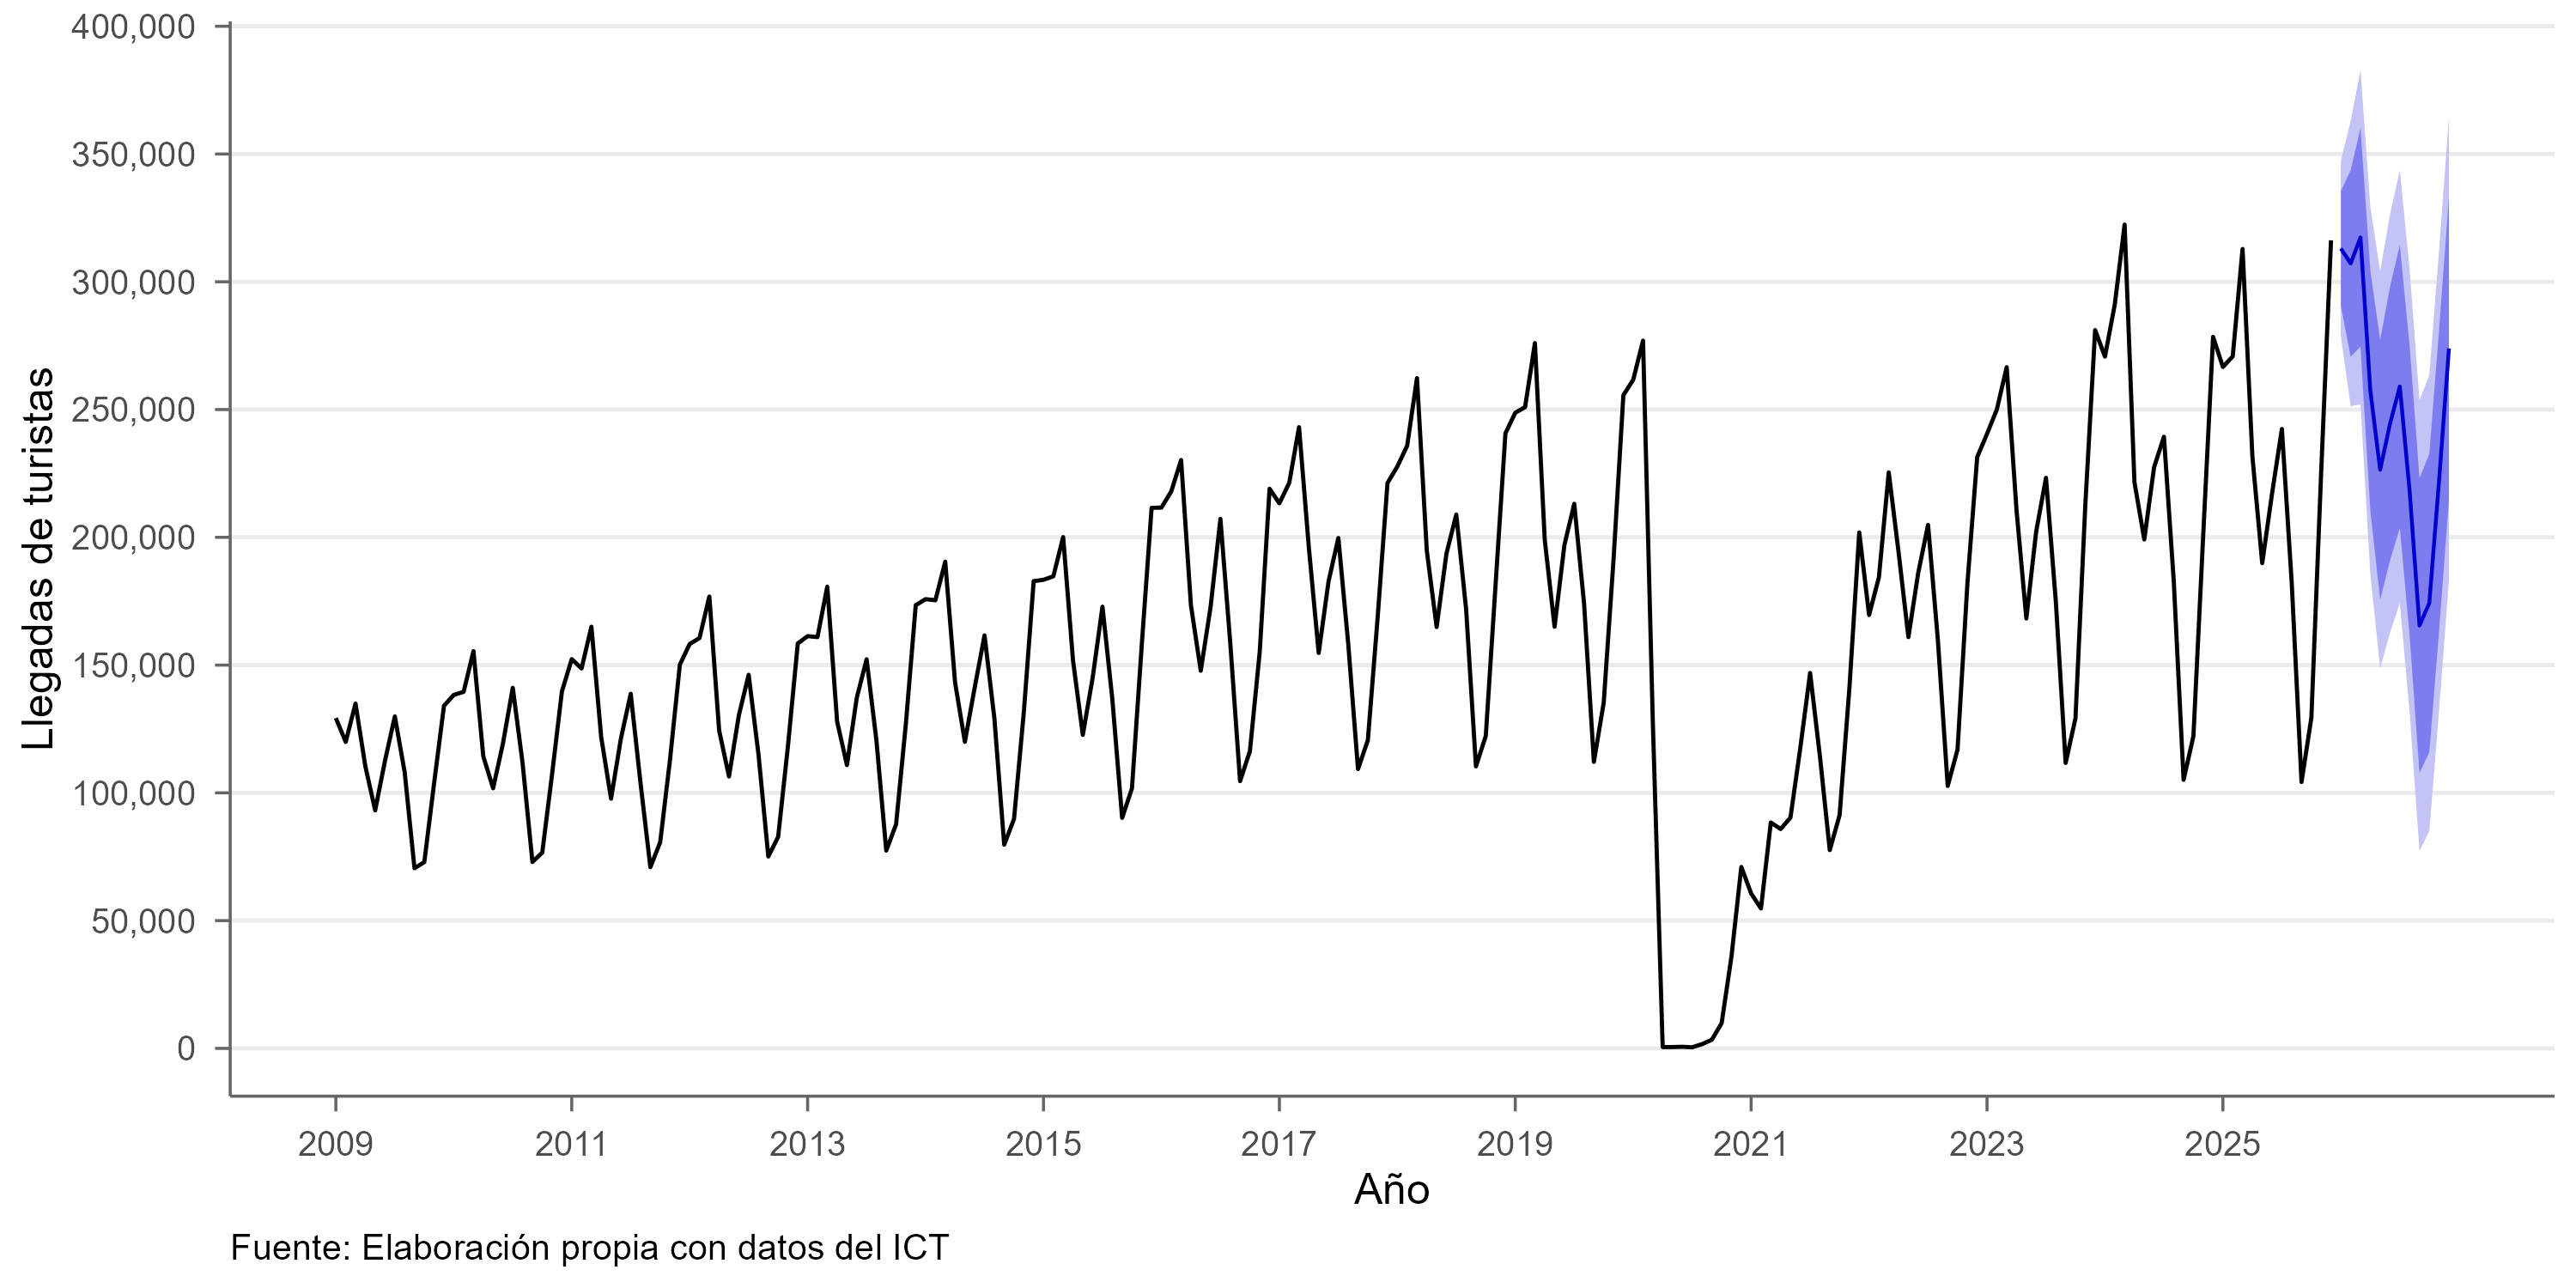
\includegraphics[width=\textwidth]{figura10.png}
    \caption{Pronósticos mensuales de llegadas de 
    turistas por vía aérea para 2026, con intervalos 
    de predicción del 80\,\% y 95\,\%.}
    \label{fig:pronostico_final}
\end{figure}

En la Figura \ref{fig:pronostico_final} se observa 
que el modelo conserva el comportamiento estacional 
de la serie. Asimismo, la amplitud de los intervalos 
de predicción aumenta conforme se incrementa el 
horizonte de pronóstico, reflejando una mayor 
incertidumbre sobre las observaciones futuras.

No obstante, debido al incumplimiento del supuesto 
de normalidad y a los indicios de variabilidad no 
constante de los residuos, los intervalos de 
predicción deben interpretarse con cautela.

\section{Conclusiones}

A partir de la comparación de las cuatro familias de 
modelos de series temporales, se concluye que la 
regresión dinámica con tendencia lineal, estacionalidad 
mensual y errores ARIMA$(4,0,0)$ fue la alternativa 
con mayor capacidad predictiva para las llegadas 
internacionales de turistas por vía aérea a Costa Rica 
durante el periodo de prueba evaluado.

El modelo presentó los menores valores de RMSE, MAE, 
MAPE y MASE, destacando un error porcentual absoluto 
medio del 10,55\,\% fuera de muestra. Asimismo, la 
incorporación de una estructura autorregresiva en 
el término de error permitió representar la 
dependencia temporal que no fue capturada por la 
regresión convencional.

Los pronósticos obtenidos para 2026 conservan el 
comportamiento estacional identificado en la serie 
histórica. Se estimó un total anual de aproximadamente 
2.979.040 llegadas de turistas por vía aérea, con 
los mayores niveles de visitación durante los 
primeros meses del año y los menores durante 
septiembre y octubre.

Entre las principales limitaciones del estudio se 
encuentra el comportamiento extraordinario de la 
serie durante la pandemia por COVID-19. Aunque se 
evaluaron modelos con variables de intervención, 
estos no proporcionaron un diagnóstico residual 
superior al del modelo seleccionado. Asimismo, la 
falta de normalidad y los indicios de variabilidad 
no constante de los residuos constituyen limitaciones 
para la interpretación de los intervalos de predicción.

Otra limitación corresponde a la evaluación predictiva 
sobre un único conjunto de prueba de doce meses, 
por lo que los resultados no garantizan que el modelo 
seleccionado mantenga su superioridad en otros 
periodos de evaluación.

Para futuras investigaciones se recomienda incorporar 
variables explicativas externas, tales como indicadores 
económicos, costos del transporte aéreo, capacidad 
aeroportuaria e indicadores de seguridad ciudadana, 
como la cantidad mensual de homicidios. La inclusión 
de estas variables permitiría evaluar si las condiciones 
económicas y de seguridad del país contribuyen a explicar 
las variaciones en las llegadas internacionales de 
turistas y a mejorar la capacidad predictiva de los 
modelos. Además, se sugiere evaluar otras 
estructuras de intervención, utilizar procedimientos 
de validación cruzada para series temporales y 
explorar métodos de construcción de intervalos de 
predicción que no dependan estrictamente del supuesto 
de normalidad.

Finalmente, los pronósticos obtenidos pueden servir 
como insumo para la planificación de la actividad 
turística, la asignación de recursos y la toma de 
decisiones en el sector turístico costarricense.































\section*{Referencias}

\begin{hangparas}{0.5in}{1}

Chou Chen, S. W. (s. f.). 
\textit{Análisis de series temporales (XS-0127)}
[Materiales didácticos del curso]. 
Escuela de Estadística, Universidad de Costa Rica.
\url{https://swchouchen.github.io/series/}

Hyndman, R. (2026). \textit{fpp2: Data for 
``Forecasting: Principles and Practice'' (2nd Edition)} 
(versión 2.5.1) [Paquete de R].
\url{https://doi.org/10.32614/CRAN.package.fpp2}

Hyndman, R., Athanasopoulos, G., Bergmeir, C., 
Caceres, G., Chhay, L., O'Hara-Wild, M., 
Petropoulos, F., Razbash, S., Wang, E., \& Yasmeen, F. 
(2026). \textit{forecast: Forecasting functions for time 
series and linear models} (versión 9.0.2) [Paquete de R].
\url{https://doi.org/10.32614/CRAN.package.forecast}

Hyndman, R. J., \& Khandakar, Y. (2008). 
Automatic time series forecasting: The forecast package 
for R. \textit{Journal of Statistical Software, 27}(3), 
1--22.
\url{https://doi.org/10.18637/jss.v027.i03}

Instituto Costarricense de Turismo. (s. f.).
\textit{Llegadas internacionales de turistas}
[Tablero interactivo de Power BI].
Departamento de Estadística Turística.
\url{https://app.powerbi.com/view?r=eyJrIjoiZGFjYTI5NTAtYmRiNy00ZjQ2LTk5ZDYtZGY2N2Q0YWNjNzcyIiwidCI6ImQwN2I2NTM1LTFkZGMtNDA2YS04MzQxLTBiMGEzMDlkNDExNSIsImMiOjR9}

Instituto Costarricense de Turismo. (2021, 13 de enero). 
\textit{Costa Rica muestra un repunte gradual en 
visitación turística al finalizar el 2020}.
\url{https://www.ict.go.cr/es/noticias-destacadas/1828-costa-rica-muestra-un-repunte-gradual-en-visitaci%C3%B3n-tur%C3%ADstica-al-finalizar-el-2020.html}

Instituto Costarricense de Turismo. (2025, 16 de enero). 
\textit{Costa Rica recibió 2,6 millones de turistas 
durante el 2024}.
\url{https://www.ict.go.cr/es/noticias-destacadas/2397-costa-rica-recibio-2-6-millones-de-turistas-durante-el-2024.html}

Nguyen, Q. H. (2025). The reciprocal impact between air 
passenger transport and international tourism in Singapore. 
\textit{Journal of Air Transport Management, 129}, 102877.
\url{https://doi.org/10.1016/j.jairtraman.2025.102877}

Organisation for Economic Co-operation and Development. 
(2024). \textit{OECD tourism trends and policies 2024}. 
OECD Publishing.
\url{https://doi.org/10.1787/80885d8b-en}

R Core Team. (2025). 
\textit{R: A language and environment for statistical 
computing} (versión 4.5.1) [Software]. 
R Foundation for Statistical Computing.
\url{https://www.R-project.org/}

Stoffer, D. (2026). 
\textit{astsa: Applied Statistical Time Series Analysis} 
(versión 2.5) [Paquete de R].
\url{https://doi.org/10.32614/CRAN.package.astsa}

Trapletti, A., \& Hornik, K. (2026). 
\textit{tseries: Time Series Analysis and Computational 
Finance} (versión 0.10-63) [Paquete de R].
\url{https://doi.org/10.32614/CRAN.package.tseries}

Vergori, A. S. (2017). Patterns of seasonality and 
tourism demand forecasting. 
\textit{Tourism Economics, 23}(5), 1011--1027.
\url{https://doi.org/10.1177/1354816616656418}

Wickham, H. (2016). 
\textit{ggplot2: Elegant graphics for data analysis}. 
Springer-Verlag.
\url{https://ggplot2.tidyverse.org}

\end{hangparas}



\clearpage

\section*{Anexos}

El código reproducible y los datos utilizados en esta 
investigación se encuentran disponibles en el siguiente 
repositorio de GitHub:

\begin{center}
\url{https://github.com/DavidBrenesCR/Pronostico-Turismo-Costa-Rica}
\end{center}

El repositorio contiene el código en R Markdown 
correspondiente al análisis exploratorio, la estimación 
y selección de los modelos, el diagnóstico residual, 
la evaluación predictiva y la generación de pronósticos. 
Asimismo, incluye los datos utilizados y el enlace 
a su fuente original.











\end{document}
